\documentclass[twocolumn]{article}
\usepackage{multicol}
\usepackage[affil-it]{authblk}
\usepackage{amsmath}
\usepackage{tcolorbox}
\usepackage{float}
\makeatletter
\newcommand{\vo}{\vec{o}\@ifnextchar{^}{\,}{}}
\makeatother
\usepackage{graphicx}
\setlength{\parindent}{4mm}
\setlength{\parskip}{0mm}
\renewcommand{\baselinestretch}{1.3}
\begin{document}
%##############################################
%TITLE PAGE
\title{Quantum Tunneling of Wave Packets in One Dimension}
\author{Andrew Crossman}
\affil{Department of Physics and Astronomy, University of Delaware}
\date{May 19th, 2019}
\maketitle
\newpage
\twocolumn[
\begin{@twocolumnfalse}
%###############################################
%ABSTRACT
%###############################################
\begin{abstract}
 This paper examines the transmissions and reflections of traveling wave packets at that undergo quantum phenomena when they come into contact with potential wells or barriers. The maximum transmission coefficients of the waves are computed as a function of both barrier/well depth, potential, and wave propagation speed in four different schemes: (1) no potential present, (2) a single barrier with varying depth, (3) two barriers with varying wave propagation, and (4) a single potential well with varying depth. In conclusion, the study finds that all three properties (barrier/well potential, depth, and wave propagation speed) and greatly effect the transmission and reflection coefficients.
\end{abstract}
\vspace{5mm}
\end{@twocolumnfalse}
]
%###############################################
%INTRODUCTION
%###############################################
\section{Introduction} 
\hspace{\parindent} Prior to the early 20th century, the world as we know it was described through the laws of classical physics which fundamentally explain natural phenomena on a macroscopic level. As technology and science developed, and physicists were able to more closely study the microscopic world however, numerous observations that could not be reconciled with classical physics began to appear, revealing that new theory and physics were needed. Among some of the most famous observations that refuted the laws of classical physics were Planck's solution to the black-body radiation problem, Einstein's photoelectric effect, and the quantum tunneling of wavelike particles through potential barriers. A very notable property of what would later be described as quantum mechanics, quantum tunneling allows for wavelike particles to 'tunnel' directly through potential barriers even if the potential energy of the barrier is greater than the kinetic energy of the incident wave! This fascinating phenomena is extremely important because it powers natural processes such as nuclear fusion in stars, radioactive decay, and astro-chemistry in interstellar clouds, and man-made devices such as tunnel junctions and transistors. 

	The physical explanation for the unexpected nature of quantum tunneling can be derived directly from the Heisenberg uncertainty principle, which states that the more precisely we know the position of a particle, the less we know about its momentum. In the context of this paper the momentum is well defined so, the more precisely a wavelike particle's momentum is calculated the greater the region it is likely to actually exist in. Fortunately, this region can be described as a probability wave function that is generally denoted as $\psi$ such that:
\begin{equation}
	1=\int_{-\infty}^{\infty} \psi^* \psi dx
\end{equation}
Hence, the crux of the explanation behind quantum tunneling is that the position of the wavelike particle cannot be exactly known, so as the particle approaches a potential barrier there begins to exist a non-zero probability that the particle is actually on the other side of the potential barrier!
%###############################################
%Methodology
%###############################################
\section{Methodology}
\hspace{\parindent}This paper explores and analyzes the application of the solutions to the Time Dependent Schrodinger Wave Equation (TDSE) to the phenomena of quantum tunneling in four different scenarios:
\begin{itemize}
	\item a wave that experiences no potential
	\item a wave that collides into a single potential barrier with varying depth $.	001\leq d\leq.01$
	\item a wave with varying propagation momentum $350\leq k\leq600$ that collides into two potential barriers with depths $d=.001$ and separation $L=.004$
	\item a wave that experiences a potential well with varying depth $.001\leq d\leq.01$
\end{itemize}
In each of these scenarios the wave packet $\psi$ is initially described as:
\begin{equation}
	\psi(x,t=0)=\frac{1}{\left(2\pi\sigma^2\right)^{1/4}}e^{\frac{-(x-x_0)^{2}}{4\sigma^2}}e^{ik_0(x-x_0)}
\end{equation}
where $\sigma$ is the width of the wave, $x_0$ is the center of the wave, and $k_0$ is the wave momentum. Unless stated otherwise these values are $\sigma^2=2.5\times10^{-4}$, $x_0=0.3$, and $k_0=700$, respectively. In addition to this, each of the waves obeys the Time Dependent Schrodinger Equation:
\begin{equation}
	\frac{-\hbar^2}{2m}\frac{\partial^2\psi(x,t)}{\partial x^2}+V(x)\psi(x,t)=i\hbar\frac{\partial\psi(x,t)}{\partial t}
\end{equation}
where $m$ is the mass of the wavelike particle, $V(x)$ is the potential at position $x$, and $\psi$ is the wave function from equation $(2)$. By defining the normalization constant $x_0^2=\frac{\hbar t_0}{m}$ and by allowing $\bar{V(x)}=\frac{t_0 V(x)}{\hbar}$, equation $(3)$ can be normalized to the form:
\begin{equation}
	\frac{i}{2}\frac{\partial^2\bar{\psi}}{\partial^2 \bar{x}^2} - i\bar{V}\bar{\psi} = \frac{\partial \bar{\psi}}{\partial \bar{t}}
\end{equation}
which is the equivalent to setting $\hbar=m=1$. Note that $\hbar$, $m$ have not actually been set to one - they have just been normalized to some length
and time such that they are removed from the equation.
\subsection{Wave Propagation}
\hspace{\parindent}The method that this paper uses to numerically solve the propagation of the wave packets in each scenario as defined by equation $(4)$ is called the ''Finite-Difference Time-Domain (FDTD) Algorithm'' which operates in three steps$^{[1]}$. The first step is to separate the real and imaginary domains of the wave function from each other such that:
\begin{equation}
	\psi(x,t)=\psi_R(x,t)+j\psi_I(x,t)
\end{equation}
where $\psi_R$ is the real domain and $\psi_I$ is the imaginary domain. This step allows each component to be separately treated ''with only real-valued computations''$^{[1]}$. The second step is to define a \textit{mesh} with a ''discrete set of grid points that sample the wave function in space and time'' in order to maintain the stability of the simulation$^{[1]}$. Allowing $\Delta x$ to be the spatial separation and $\Delta t$ to be the temporal separation between each grid point, the \textit{mesh} is defined as:
\begin{align}
	x_\ell &= \ell\Delta x \\
	t_n &= n\Delta t
\end{align}
where $x_\ell$ is the current position, $\ell$ is the total distance, $t_n$ is the current time, and $n$ is the current timestep. To maintain the aforementioned stability of the system, $\Delta t$ must be less than a 'maximum allowable time
increment' defined as:
\begin{equation}
	\Delta t \leq \frac{\hbar}{\frac{\hbar^2}{m\Delta x^2}+\frac{V_0}{2}}
\end{equation}
where $\Delta t_c$ can be seen to depend on a chosen $\Delta x$ $^{[1]}$.
The final step is to update the \textit{mesh} for the length of time that the simulation takes place. To do this the derivatives for $\psi_R$ and $\psi_I$ must be approximated by using finite-differences and corrected using the central-difference method. Plugging these approximations into the partial derivatives of equation $(5)$ with respect to $R$ and $I$, then yields the following equations for $\psi_R$ and $\psi_I$: 
\begin{equation}
\begin{split}
  \psi_I^{n+\frac{1}{2}}(\ell) = &K_1[\psi_R^n(\ell+1)+\psi_R^n(\ell-1)-2\psi_R^{n}(\ell)]\\ 
  &-K_2V(\ell)\psi_R^n(\ell)+\psi_I^{n-\frac{1}{2}}(\ell)
\end{split}
\end{equation}
\begin{equation}
\begin{split}
  \psi_R^{n+1}(\ell) = &-K_1[\psi_I^{n+\frac{1}{2}}(\ell+1)\psi_I^{n+\frac{1}{2}}(\ell-1)-2\psi_I^{n+\frac{1}{2}}(\ell)]\\ 
  &+K_2V(\ell)\psi_I^{n+\frac{1}{2}}(\ell)+\psi_R^{n}(\ell)
\end{split}
\end{equation}
where the imaginary part of the wave function exists at half-step time intervals from the real part - meaning that $\psi_R^n$ and $\psi_I^{n-\frac{1}{2}}$ are the \textit{present} states of the wave function and that $\psi_R^{n+1}$ and $\psi_I^{n+\frac{1}{2}}$ are the \textit{future} states of the wave function. It should also be noted that $K_1$ and $K_2$ are defined as:
\begin{align}
	K_1 &= \frac{\hbar \Delta t}{2m\Delta x^2} = \frac{\Delta t}{2\Delta x^2}, normalized \\
	K_2 &= \frac{\Delta t}{\hbar} = \Delta t, normalized
\end{align}
\subsection{Calculating the Transmission and Reflection Coefficients}
\hspace{\parindent}Two important measurements that will be used to describe the wave packets after they collide with the potential barriers and wells in their respective scenario are the resulting transmission and reflection coefficients. These coefficients correspond directly to the probability of the position of the wavelike particle. For example, a transmission coefficient of $T=.70$ would mean that there is a 70\% probability that the particle passes through the wall, and consequently a 30\% chance that it is reflected. Numerically these quantities are very simple to calculate - simply sum the portion of the wave packet that is beyond the potential barriers/wells to find the transmission coefficient and sum the portion of the wave packet that is prior to the barriers/wells to find the reflection coefficient. Solving this problem analytically is a bit more difficult though, and requires a bit of math. Take a general solution to the Schrodinger equation for a particle approaching from the left as:
\begin{equation}
	\psi_1(x)= Ae^{ik_1x}+Be^{-ik_1x}, x<-a
\end{equation}
\begin{equation}
	\psi_2(x)= Ce^{k_2x}+De^{-k_2x}, -a<x<a
\end{equation}
\begin{equation}
	\psi_3(x)= Fe^{ik_1x}+Ge^{-ik_1x}, a<x
\end{equation}
where $k_1=\frac{\sqrt{2mE}}{\hbar}$, and $k_2=\frac{\sqrt{2m(V-E)}}{\hbar}$. Here $Ae^{ik_1x}$ represents the incident wave, $Be^{-ik_1x}$ represents the reflected wave, $Ce^{k_2x}$ represents the wave traveling to the right in the barrier/well,  $De^{-k_2x}$ represents the wave traveling to the left inside the barrier/well, $Fe^{ik_1x}$ represents the transmitted wave, and $Ge^{-ik_1x}$ has no physical significance (i.e. $G=0$). Acknowledging the fact that the wave function is continuous at the boundaries leads to the results that:
\begin{equation}
\begin{split}
	2Ae^{-ik_1a}&=\left(1-\frac{ik_2}{k_1}\right)Ce^{-k_2a} \\
	&+\left(1+\frac{k_2}{k_1}\right)De^{k_2x}
	\end{split}
\end{equation}
\begin{equation}
	Ce^{k_2a}=\frac{1}{2}\left(1+\frac{ik_1}{k_2}\right)Fe^{ika}
\end{equation}
\begin{equation}
	De^{-k_2a}=\frac{1}{2}\left(1-\frac{ik_1}{k_2}\right)Fe^{ika}
\end{equation}
By substituting equations $(17)$ and $(18)$ into equation $(16)$, A and F - the incident and transmitted wave coefficients can be isolate:
\begin{equation}
	Ae^{-ik_1a}=Fe^{ik_1a}\left[\cosh(2k_2a)+\frac{i(k_2^2-k_1^2)}{2k_1k_2}\sinh(2k_2a)\right]
\end{equation}
At this point it should be noted that due to the initial descriptions of $\psi_1$, $\psi_2$ and, $\psi_3$ that $|A|^2$ is the intensity of the incident wave, $|B|^2$ is the intensity of the reflected wave and $|F|^2$ is the intensity of the transmitted wave. Hence, the ratio of $|F|^2$ to $|A|^2$ is the transmission coefficient! Its generalized equation being:
\begin{align}
	T&=\frac{|F|^2}{|A|^2} \\
	T&=\left[1+\frac{V^2}{4E(V-E)}\sinh^2\left(\frac{2a}{\hbar}\sqrt{2m(V-E}\right)\right]^{-1}
\end{align}
And consequentially, the generalized equation reflection coefficient being:
\begin{align}
	R&=1-T \\
	R&=1-\left[1+\frac{V^2}{4E(V-E)}\sinh^2\left(\frac{2a}{\hbar}\sqrt{2m(V-E}\right)\right]^{-1}
\end{align}
Unsurprising then, the transmission and reflection coefficients clearly depend on the potential of the barrier/well, its depth, and the propagating momentum of the particle as defined by $E=k_o^2/2$ in normalized coordinates. 
\section{Verification of the Numerical Method}
\begin{figure}[ht]
\centering
\caption{Normalization of the Wave Packet When No Potential is Present}
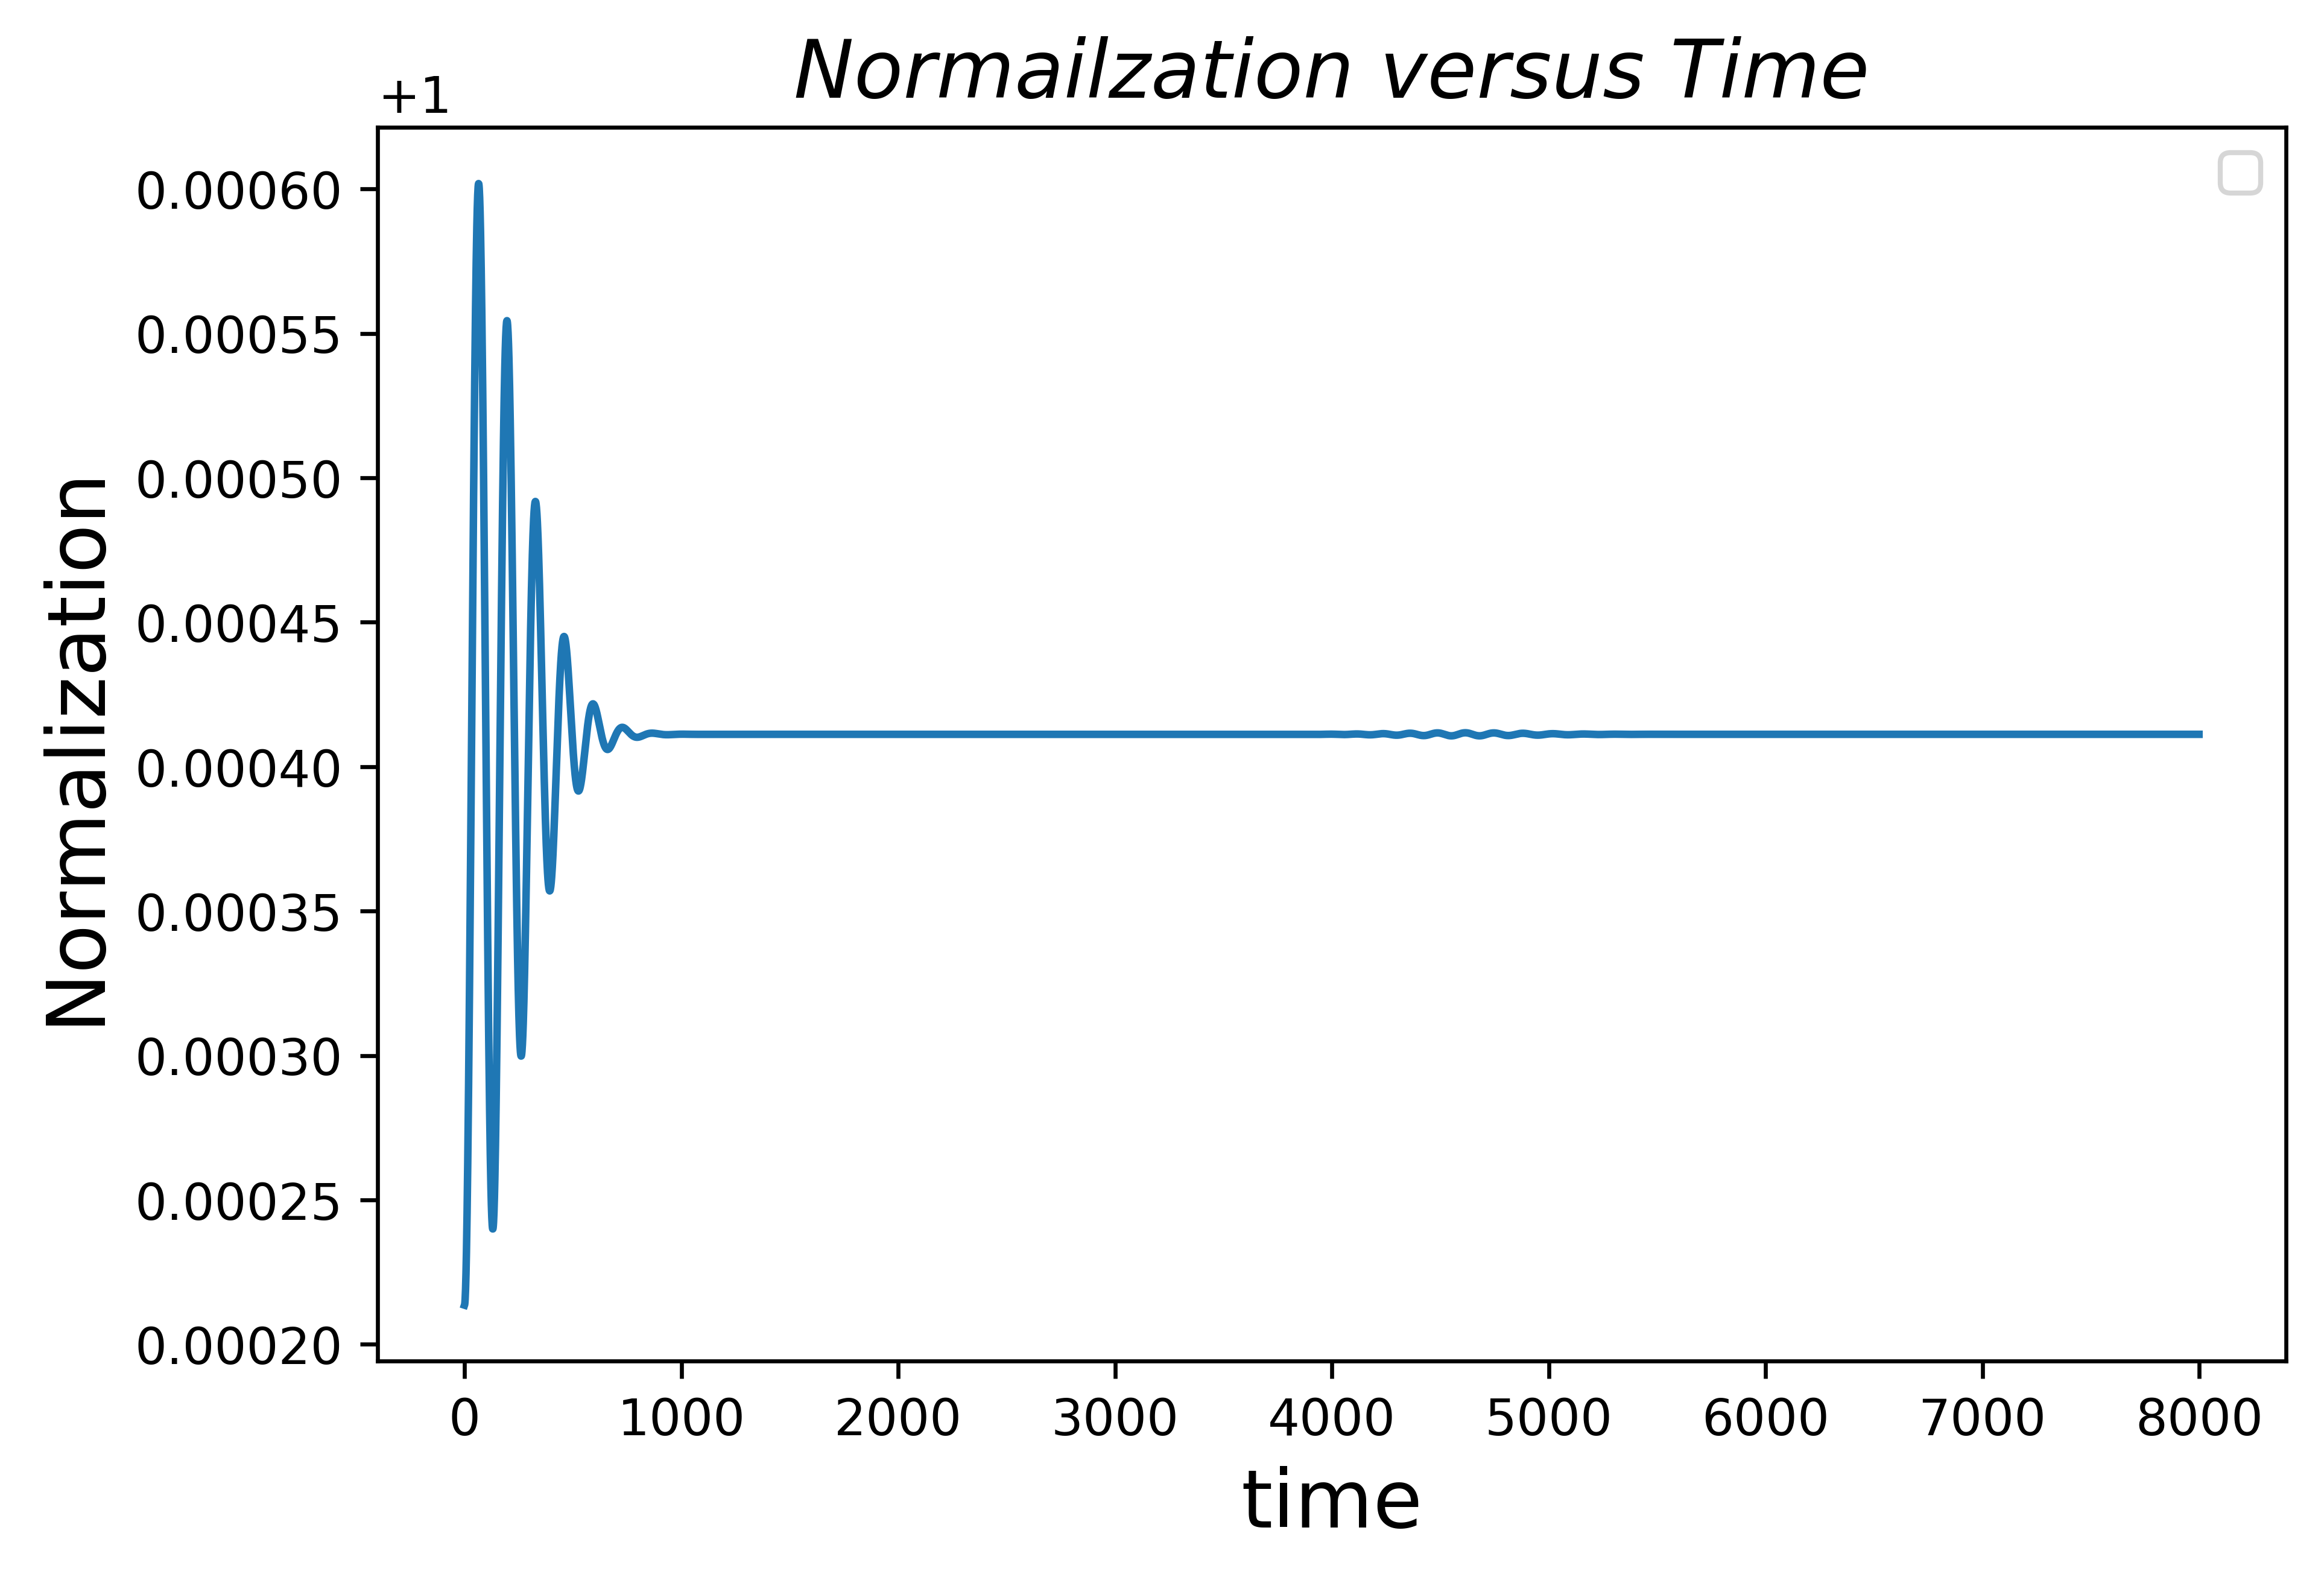
\includegraphics[scale=.5]{Norm1}
\small{This plot shows the normalization of the wave packet when V=0 for all x. At the beginning the normalization is quite erratic but it quickly stabilizes about 1 as it should according to equation $(1)$}
\end{figure}
\hspace{\parindent}The first experiment that was run using the Finite-Difference Time-Domain Algorithm as mentioned before was a simple verification of the numerical method. This experiment was performed with  no potential barriers or wells to ensure that there were no abnormalities in the methodology, such as a $\Delta t$ being used that was greater than $t_c$ which would cause exponential growth in the normalization of equation $(1)$. Fortunately, after a few minor adjustments everything was functioning fine. In order to analyze the findings some additional methods outside of the methodology described in section two were used. For example, the quantities $<x>$ and $\sigma(t)$ were measured to determine whether or not wave packet was behaving as expected. These quantities were measured using the following formulas:
\begin{align}
	<x>&=\int_{-\infty}^{\infty}\psi^*x\psi dx \\
	<x^2>&=\int_{-\infty}^{\infty}\psi^*x^2\psi dx \\
	\sigma(t)&=\sqrt{<x^2>-<x>^2}
\end{align}
where $<x>$ describes the average position of the wave packet and $\sigma(t)$ describes its average spread. Taking these into account, some points of interest for these initial tests were that:
\begin{figure}[H]
\centering
\caption{Average Wave Packet Position When No Potential is Present}
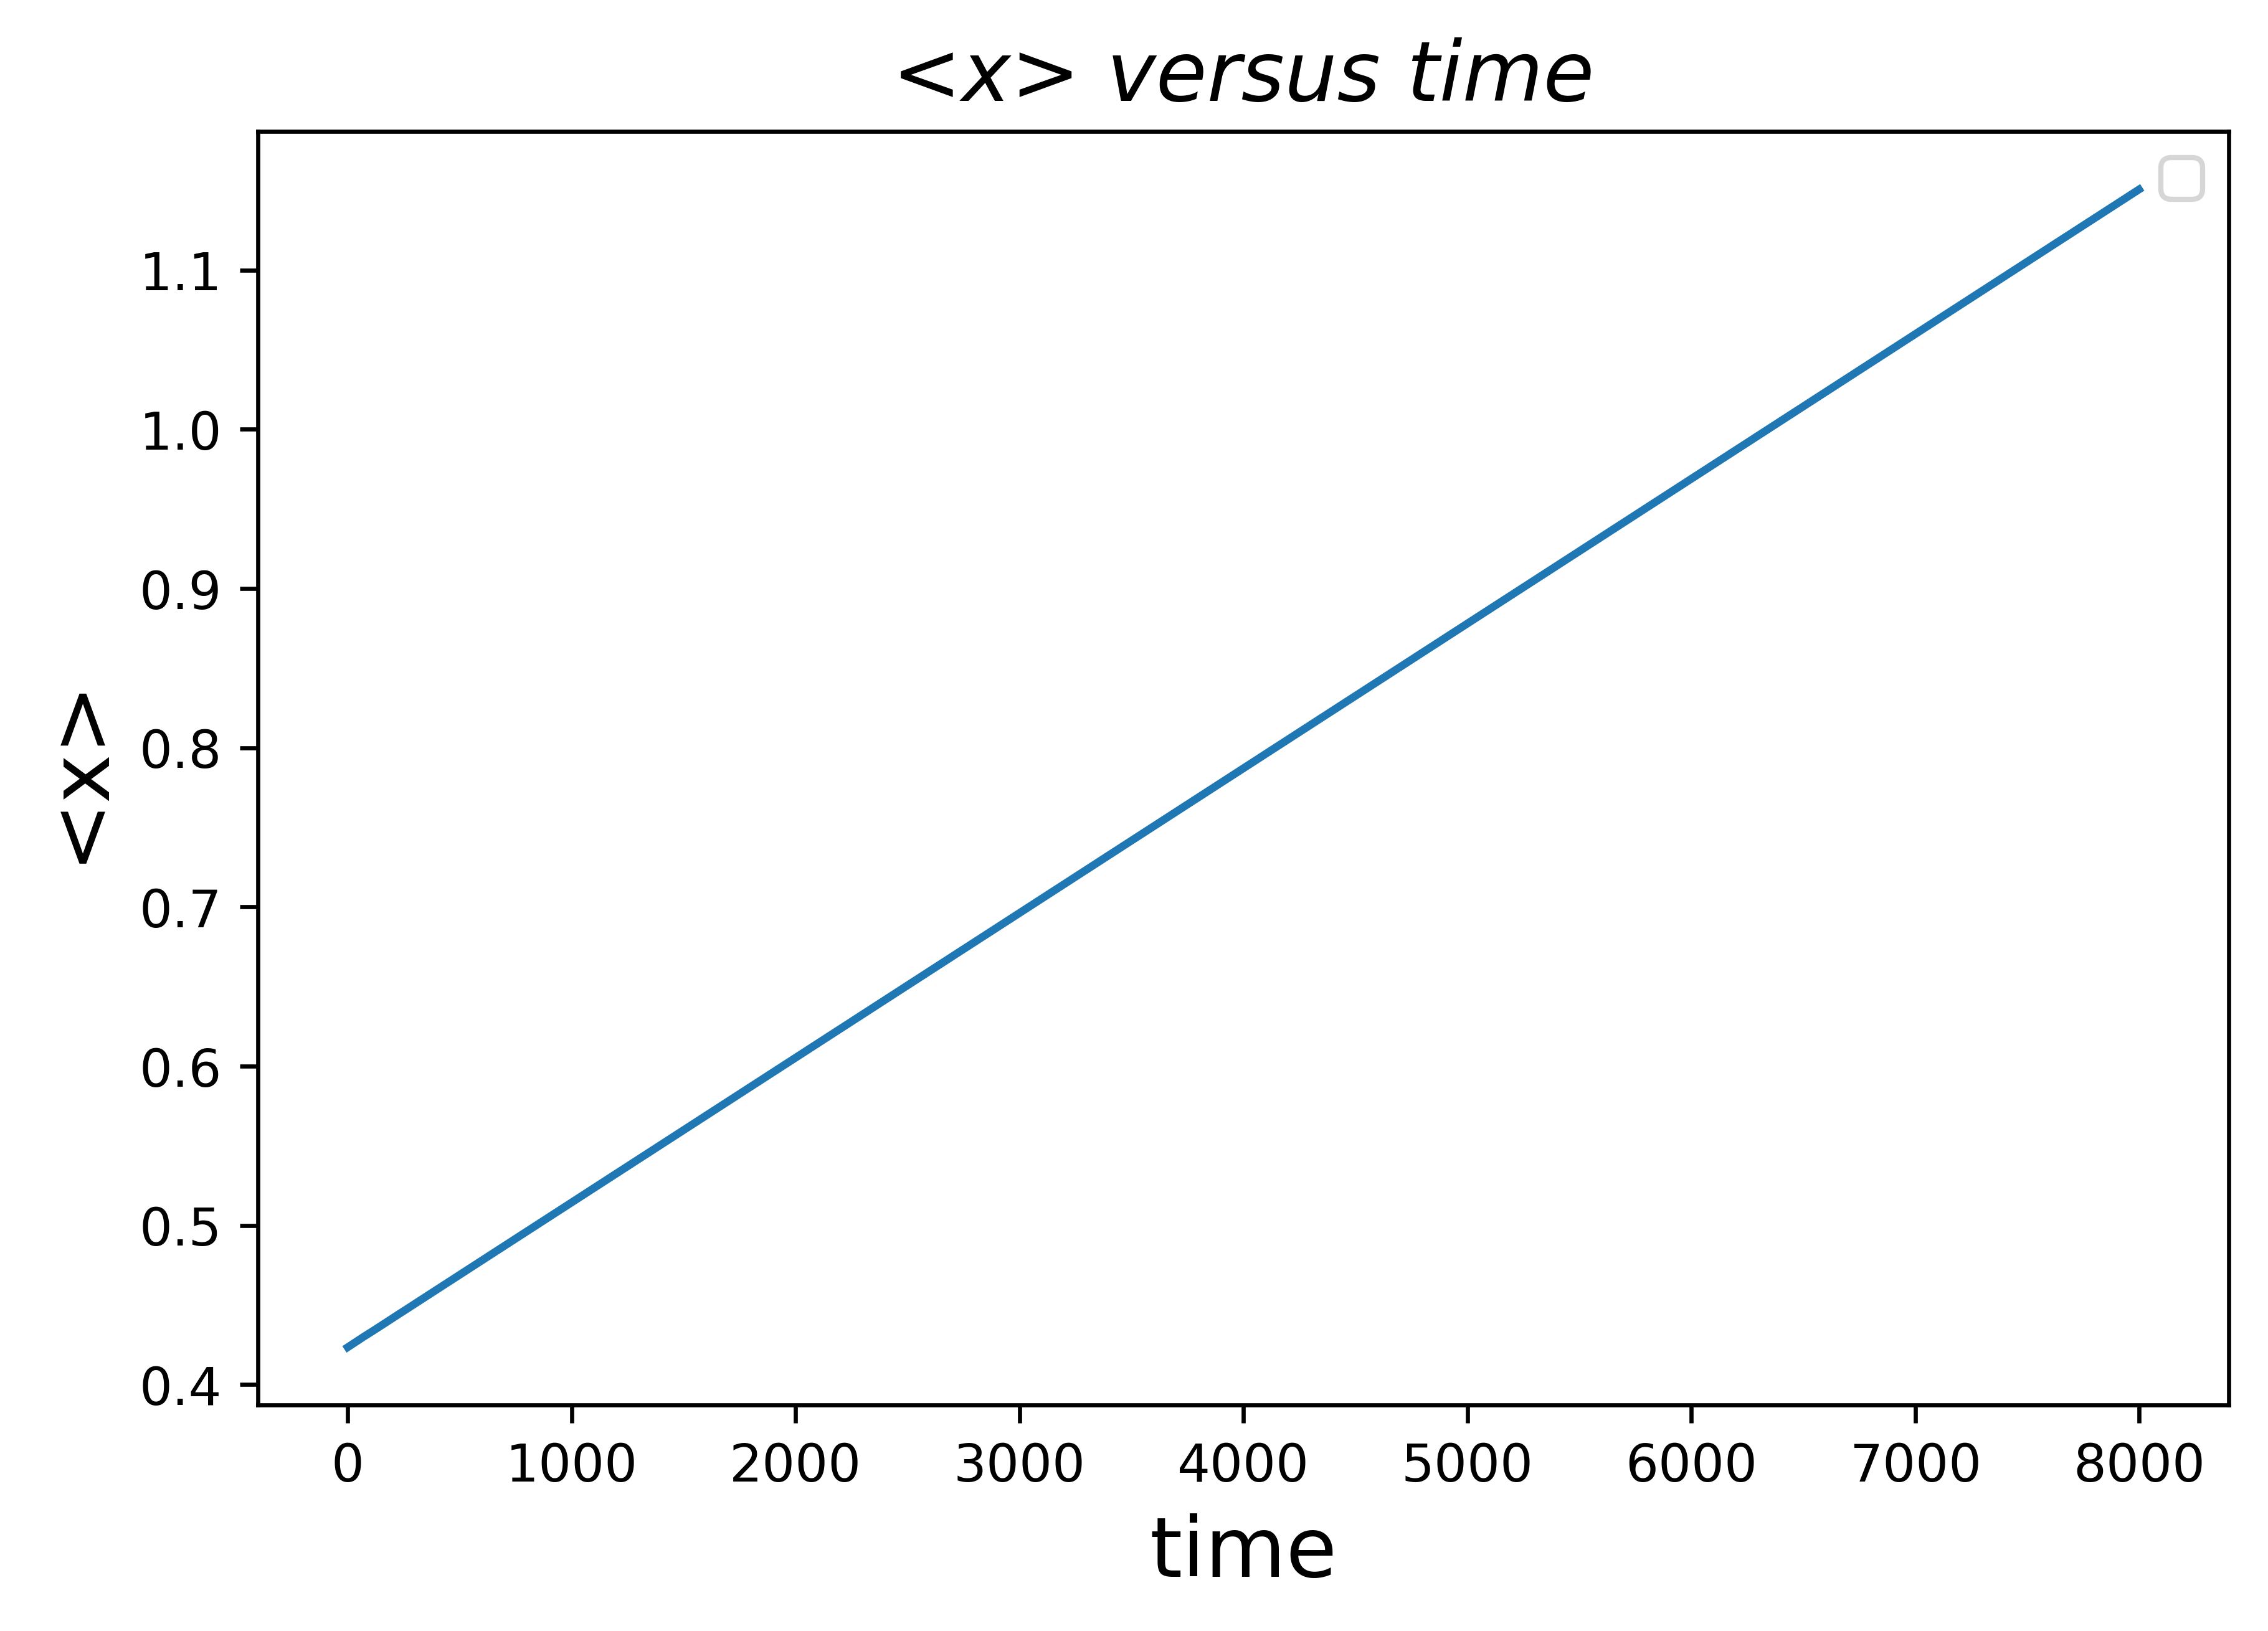
\includegraphics[scale=.5]{X1}
\small{This plot shows $<x>$ for the wave packet when V=0 for all t. It is clearly linear which it expected since the wave speed is fixed at $k_0$}
\centering
\caption{Wave Packet Spread over Time When No Potential is Present}
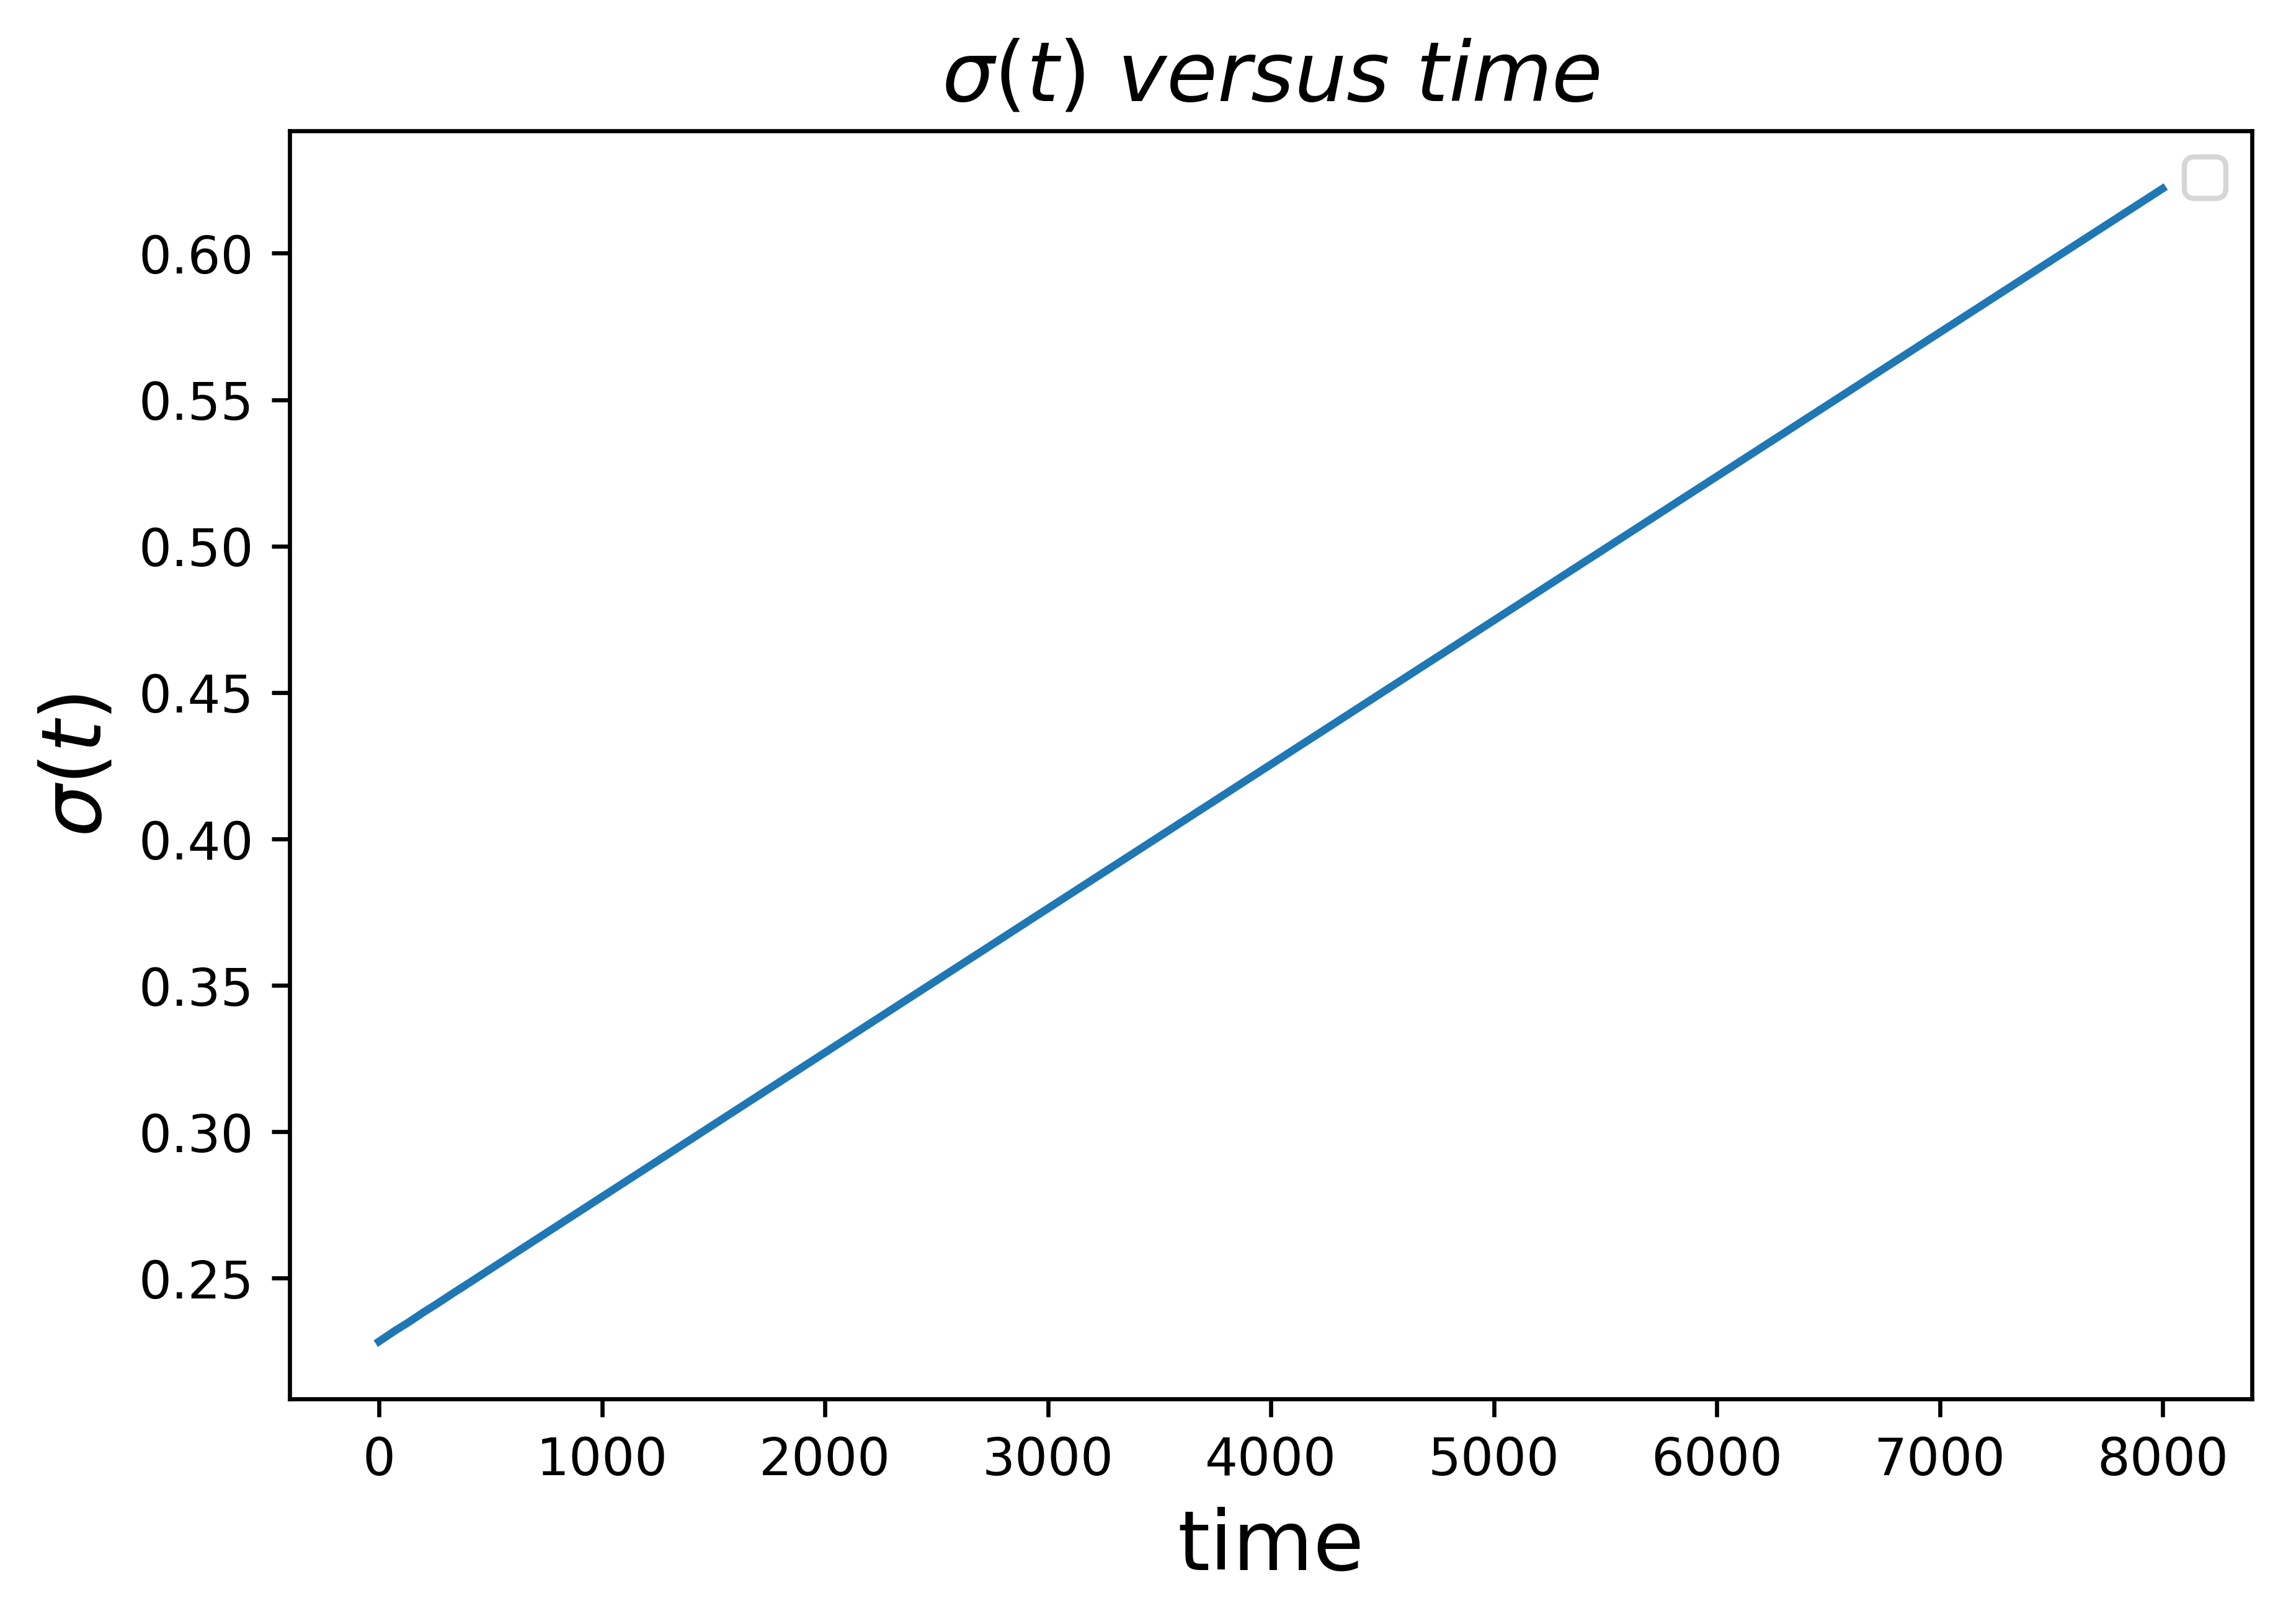
\includegraphics[scale=.5]{sigma1}
\small{This plot shows $\sigma(t)$ for the wave packet when V=0 for all t. It is clearly linear which it expected because without interference the wave should slowly spread out linearly.}
\end{figure}
\begin{itemize}
\item the normalization over time varied wildly initially, at least relative to later times but was overall very small with a range of +/- .0002 about the average (see Figure 1).
\item $<x>$ grows linearly with time, indicating that the wave packet is indeed moving at a fixed speed, $k_0$ (see Figure 2) which is expected
\item $\sigma(t)$ also increases linearly with time, indicating that the wave packet spreads out in a linear manner (see Figure 3) which is expected
\item irregardless of the initial width of the wave packet, assuming the other conditions are the same their $<x>$ and $\sigma(t)$ quantities act exactly the same (see Figures 3 and 4)
\end{itemize}
\begin{figure}[h]
\centering
\caption{Wave Packet Spread over Time for a Different Initial Distribution}
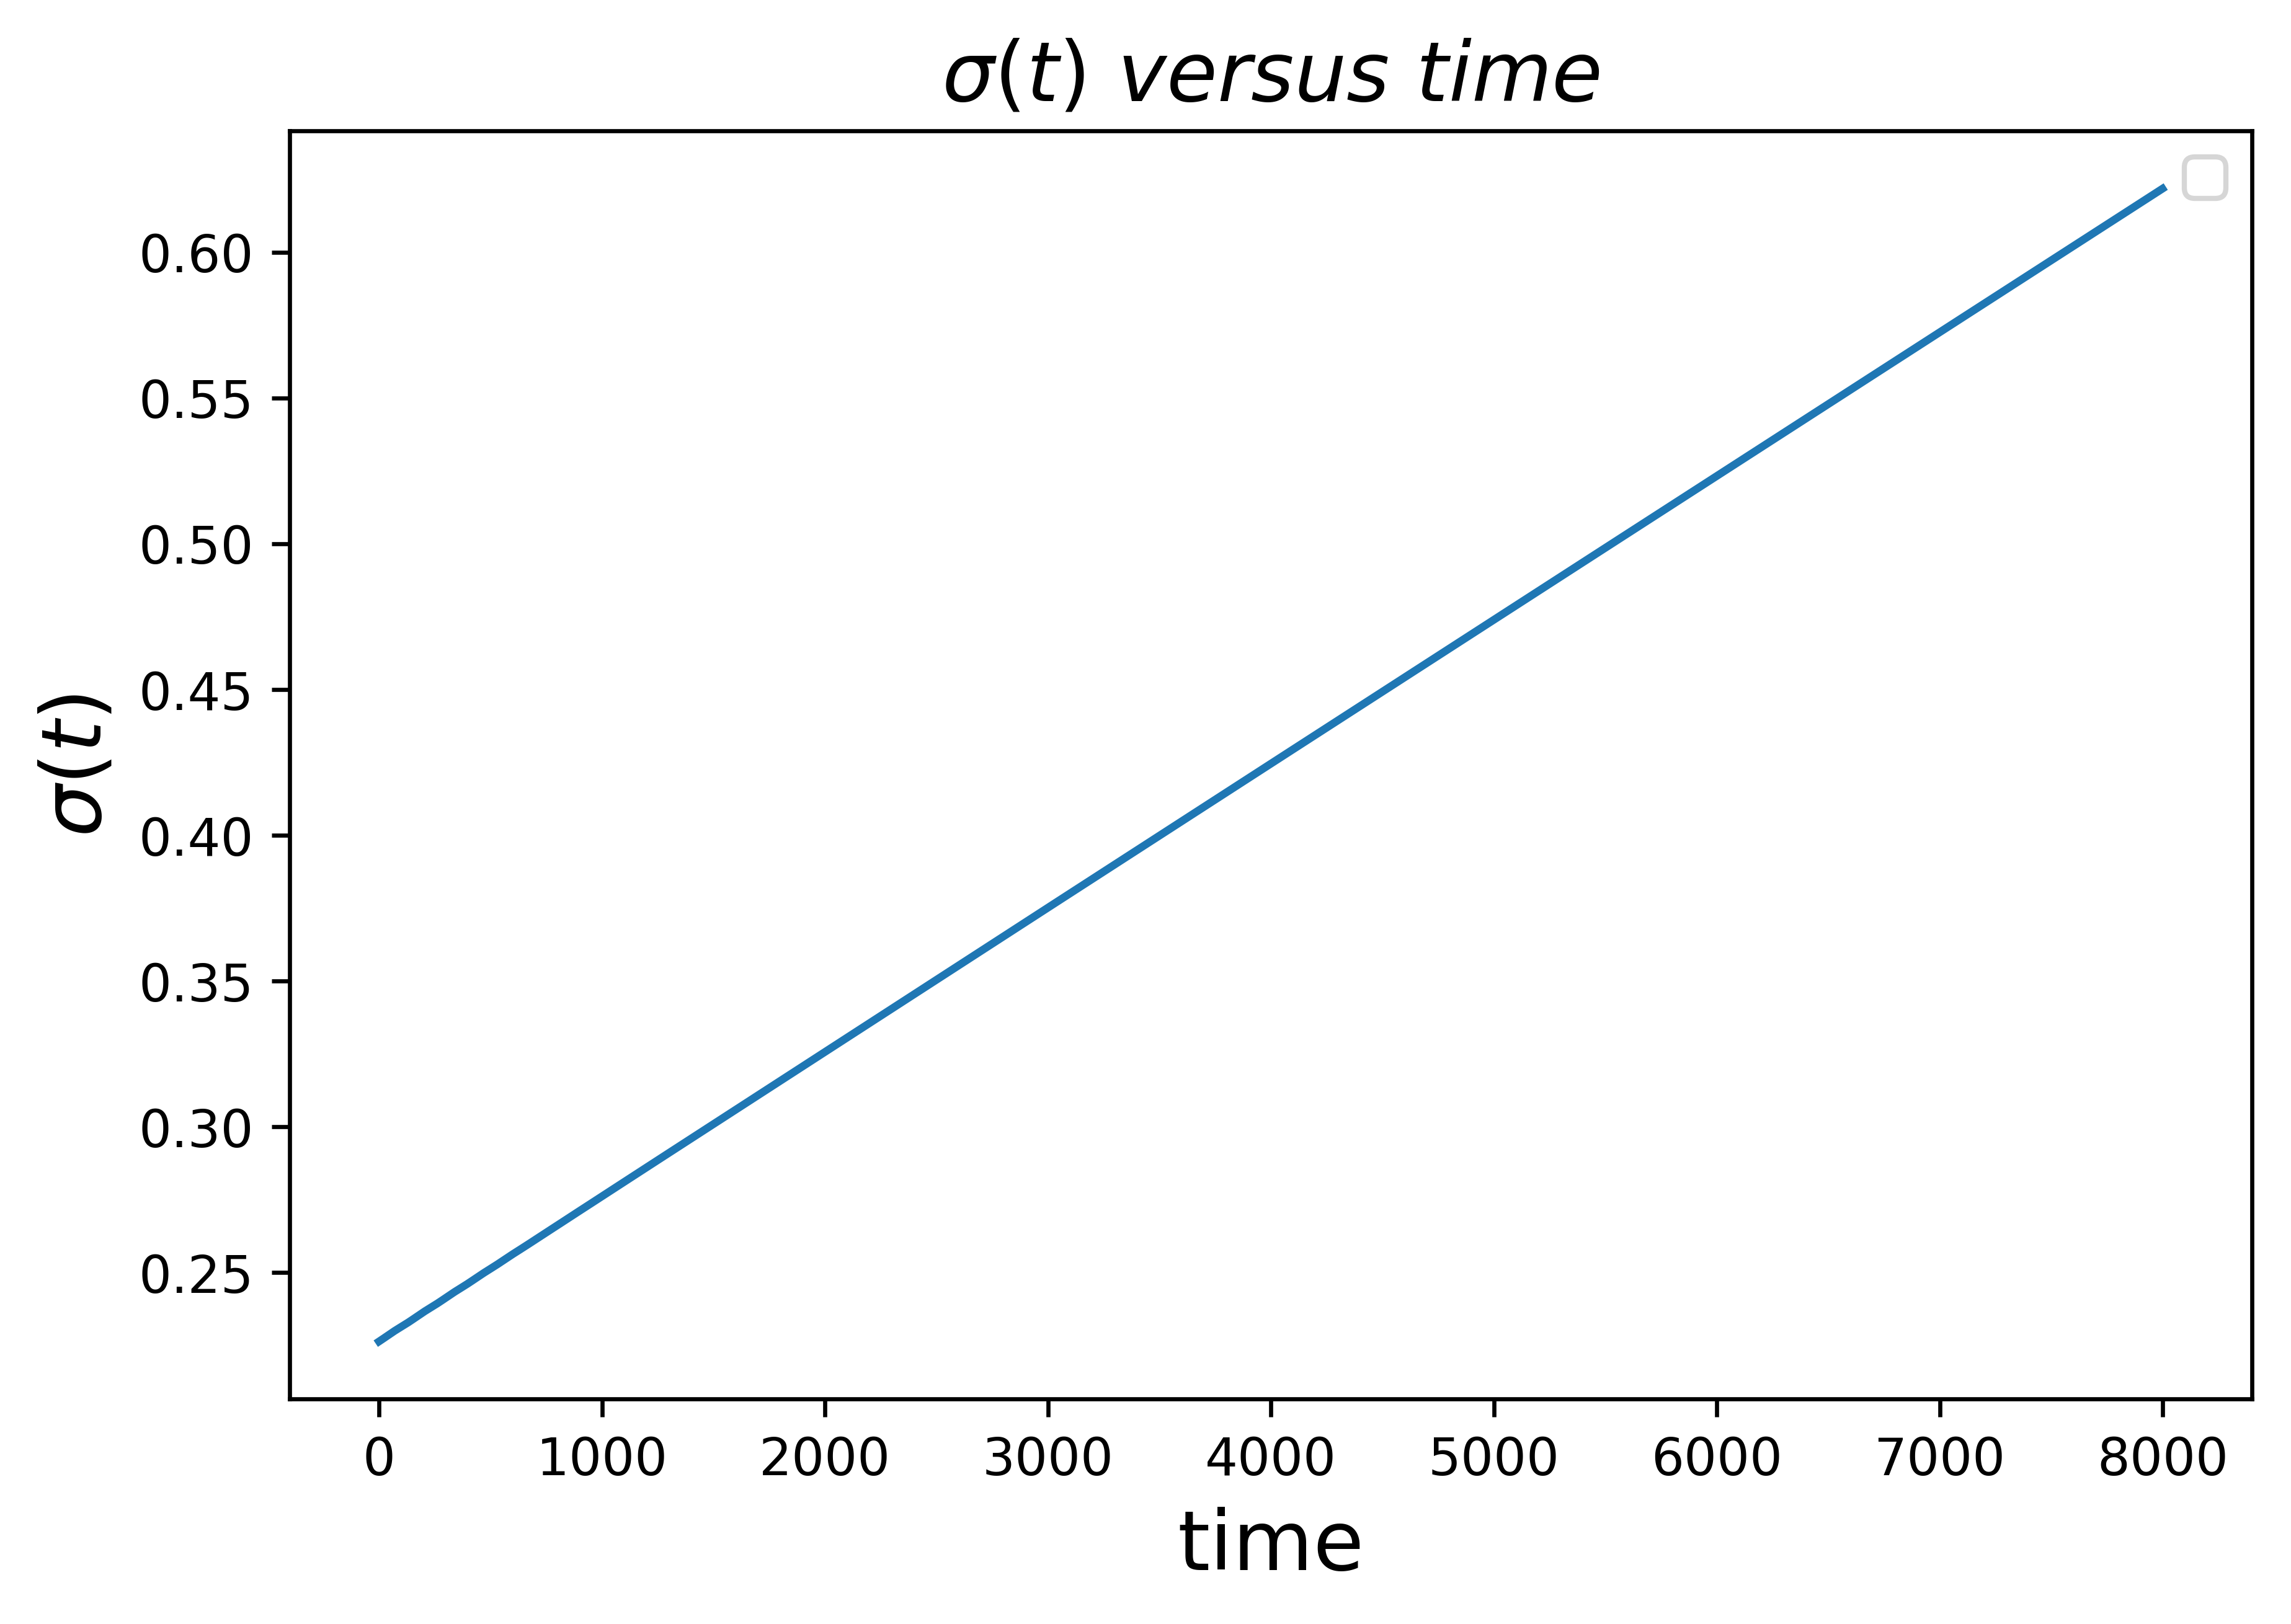
\includegraphics[scale=.5]{sigma1b}
\small{This plot shows $\sigma(t)$ for the same wave packet used in Figure 3 expect that the initial distribution has been increased to $9\times10^{-4}$ from $2.5\times10^{-4}$. The graphs are exactly identical revealing that despite the change in the initial spread they still spread out at the same rate.}
\end{figure}
%%%%%%%%%%%%%%%%%%%%%%%%%%%%%%%%%%%
% New Section
%%%%%%%%%%%%%%%%%%%%%%%%%%%%%%%%%%%
\section{Tunneling Through a Single Barrier}
\hspace{\parindent}After verifying the methodological sustainability of the system in experiment one, experiment two sought to build upon the framework by testing the wave packet against a single potential barrier. The goal here was to examine exactly how sensitive the Transmission coefficient is to the depth of the barrier. Although the analytic answer was derived in section 2.2, it is nevertheless pertinent to verify the analytic answer through physical observation - or in this case a numeric simulation. In order to do just that, the simulation with a single barrier was run several times with different depths between being used. The first simulation used a barrier depth $d=.001$ and the last a depth $d=.01$ with intervals of $\Delta d=.001$ for each simulation in between.
\begin{figure}[H]
\centering
\caption{Wave Packet over Time for a Single Potential Barrier}
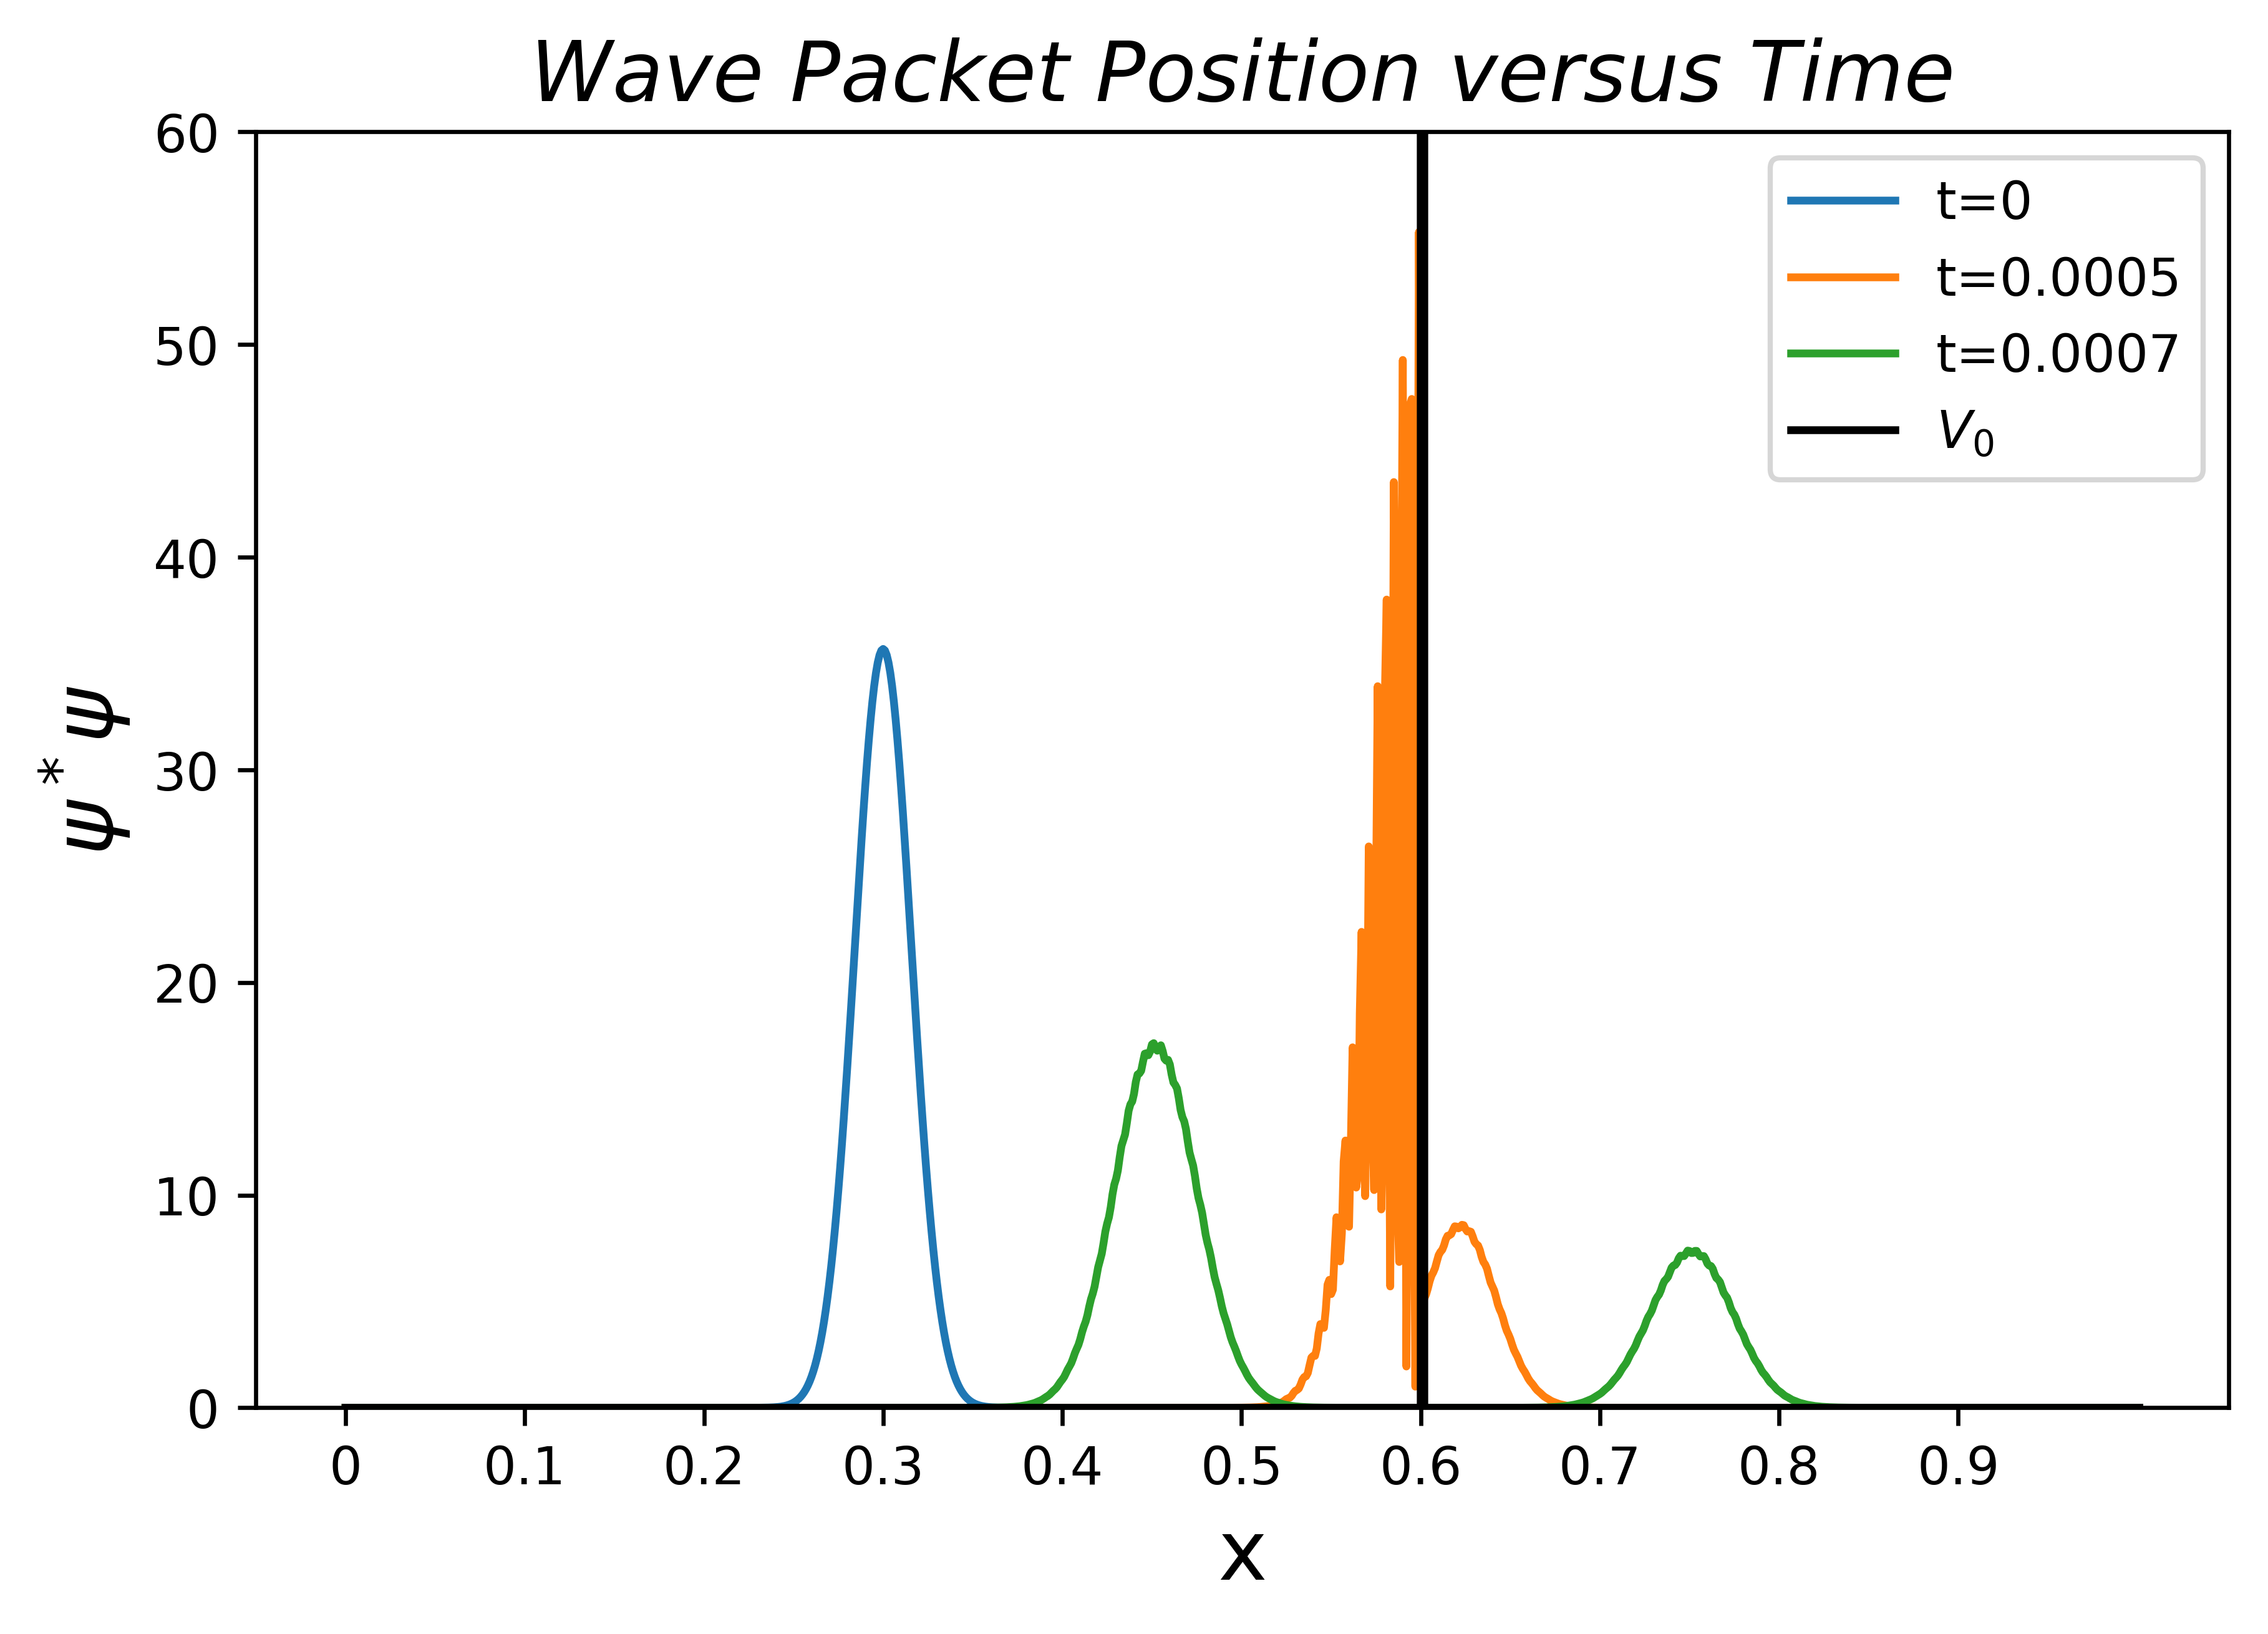
\includegraphics[scale=.5]{Position2}
\small{This plot shows the probability distribution of where the particle described by $\psi$ could be. In this case the depth of the barrier is $d=.001$ and it clearly shows that quantum tunneling has occurred.}
\end{figure}
Predictably, the first simulation revealed that a much larger portion of the wave packet was able to pass through the barrier than in the last simulation (see Figures 5 and 6). In fact, it would seem that none of the wave packet was actually able to pass through the thicker barrier at all! Plotting the numeric transmission coefficient further reveals that it actually drops off very steeply such that by $d=.004$ there is virtually no tunneling occurring (see Figure 7).
\begin{figure}[ht]
\centering
\caption{Wave Packet over Time for a Thicker Single Potential Barrier}
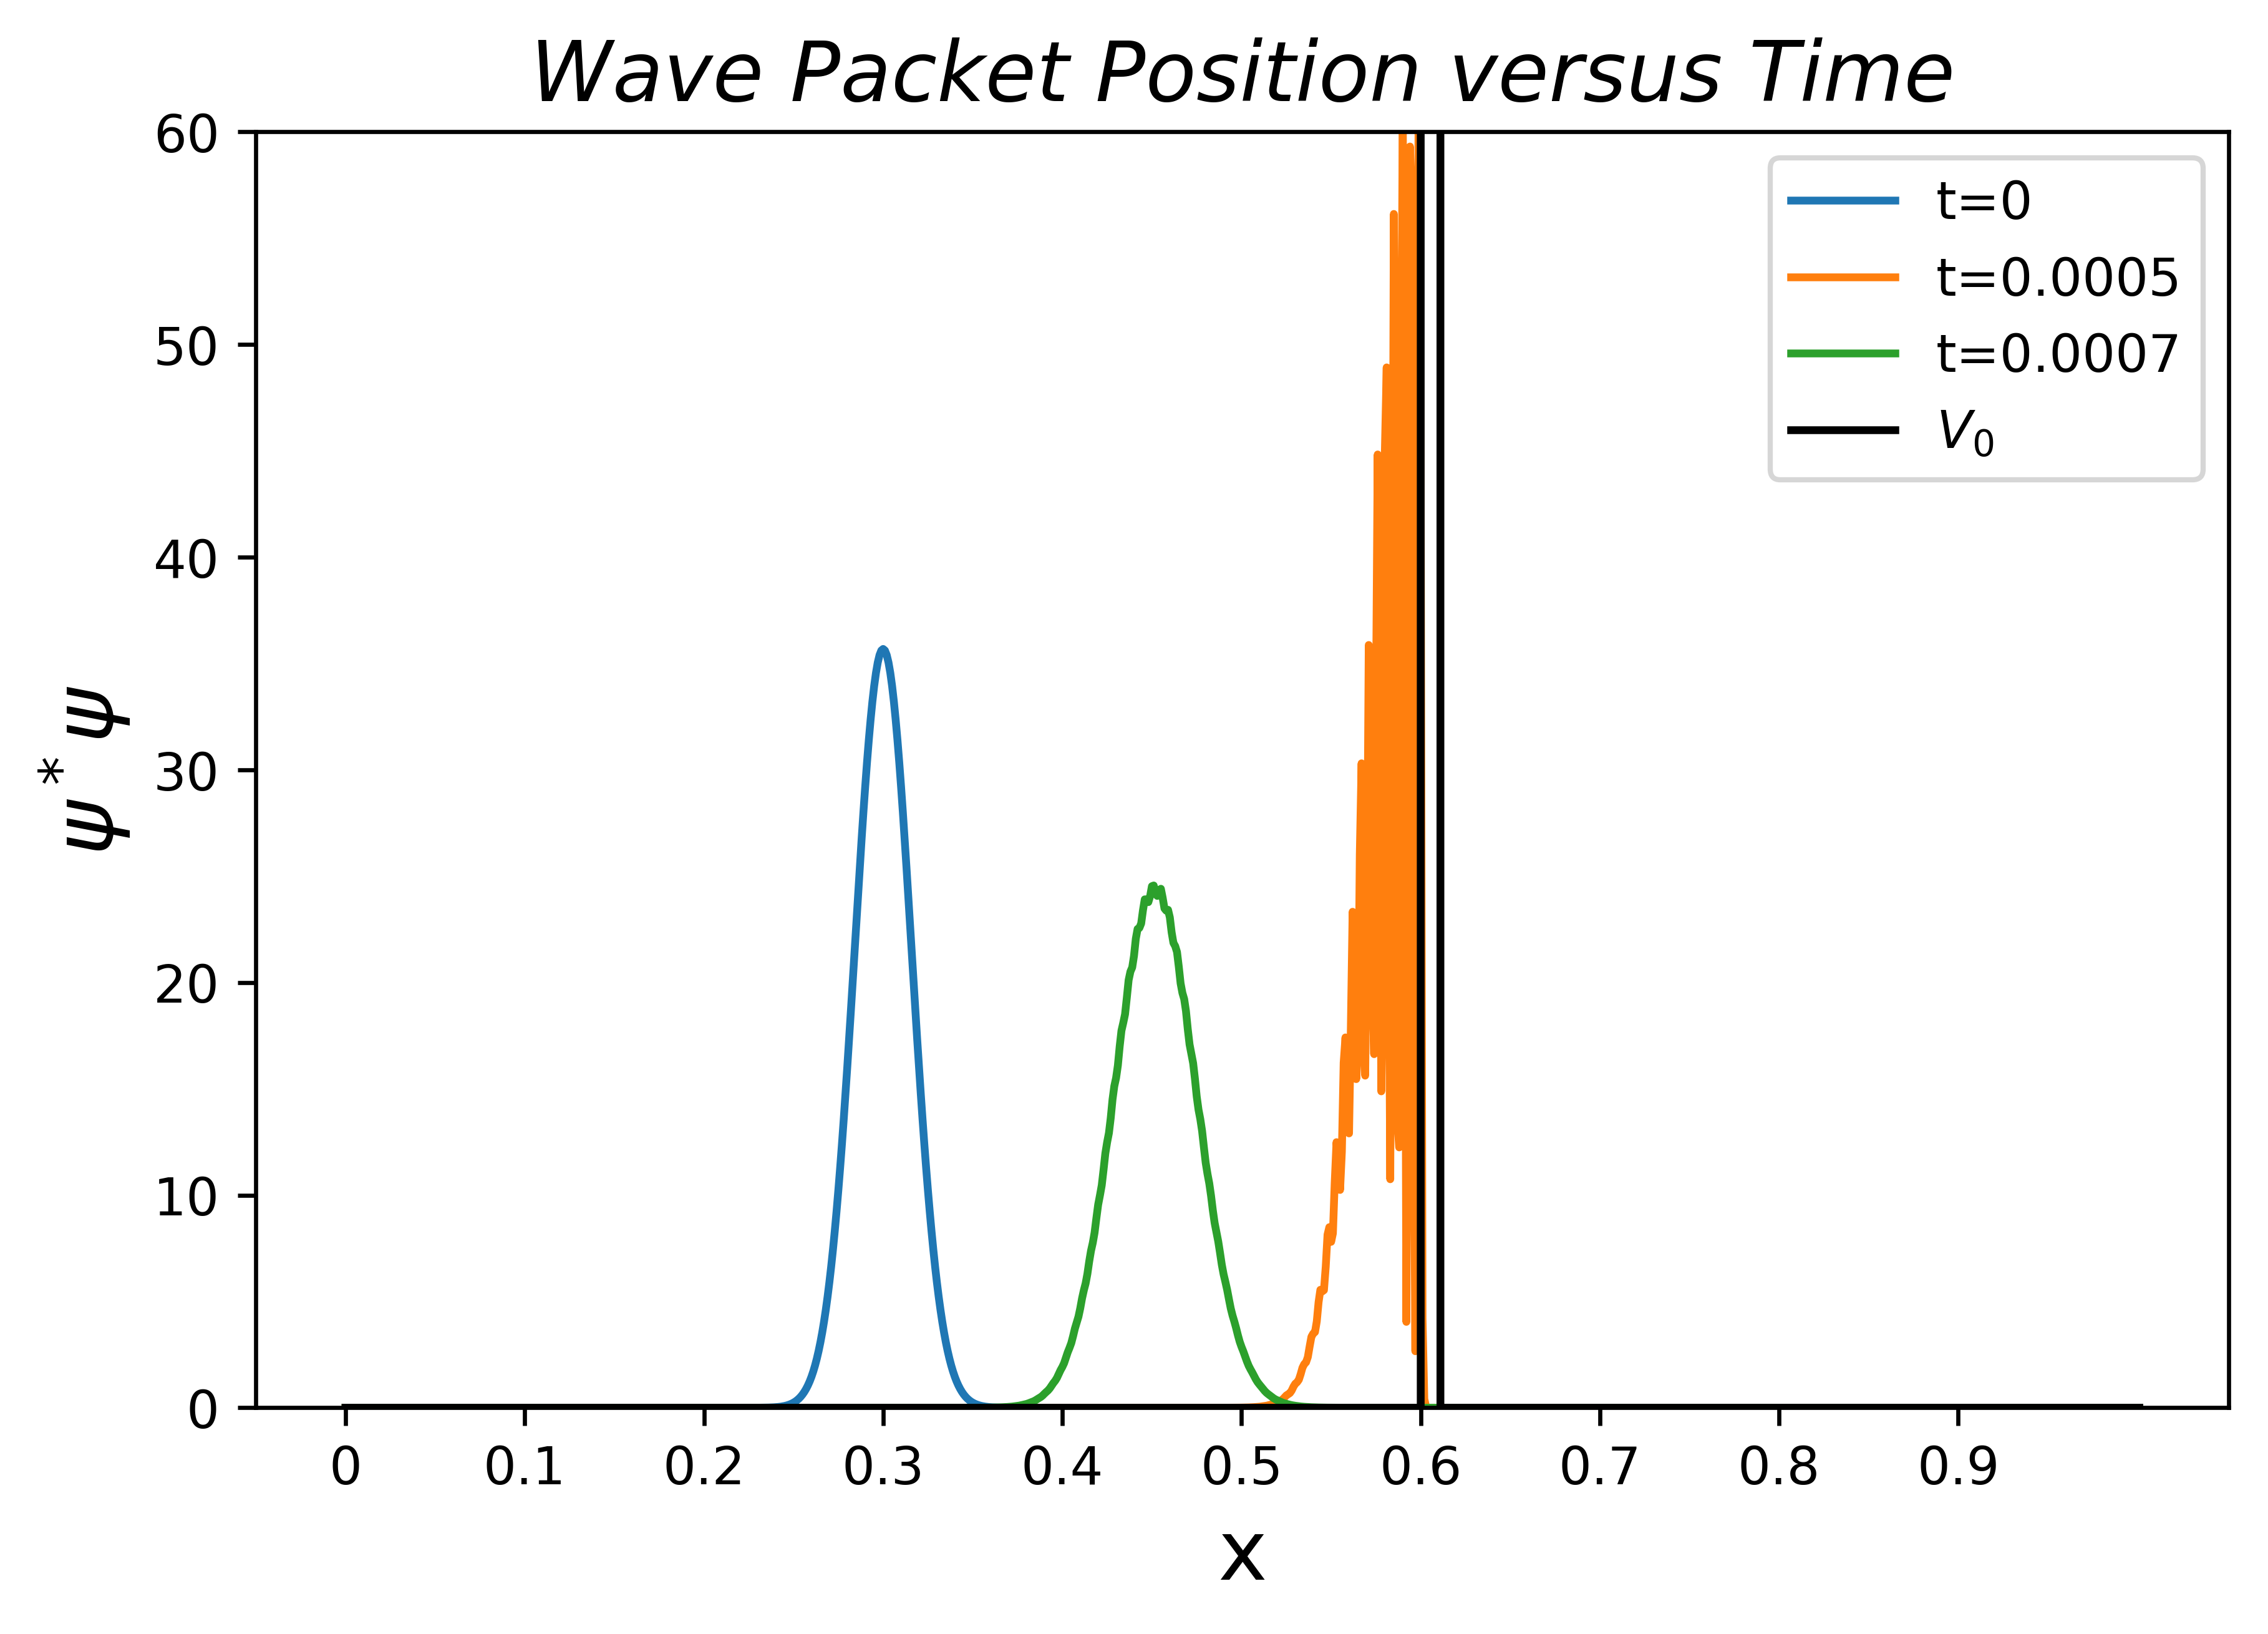
\includegraphics[scale=.5]{Position2b}
\small{This plot shows the probability distribution of where the particle described by $\psi$ could be. In this case the depth of the barrier is $d=.01$ and it shows that there is no visible probability that the particle was able to travel through the barrier.}
\end{figure}
\begin{figure}[h]
\centering
\caption{Numeric Transmission Coefficient for a Single Potential Barrier}
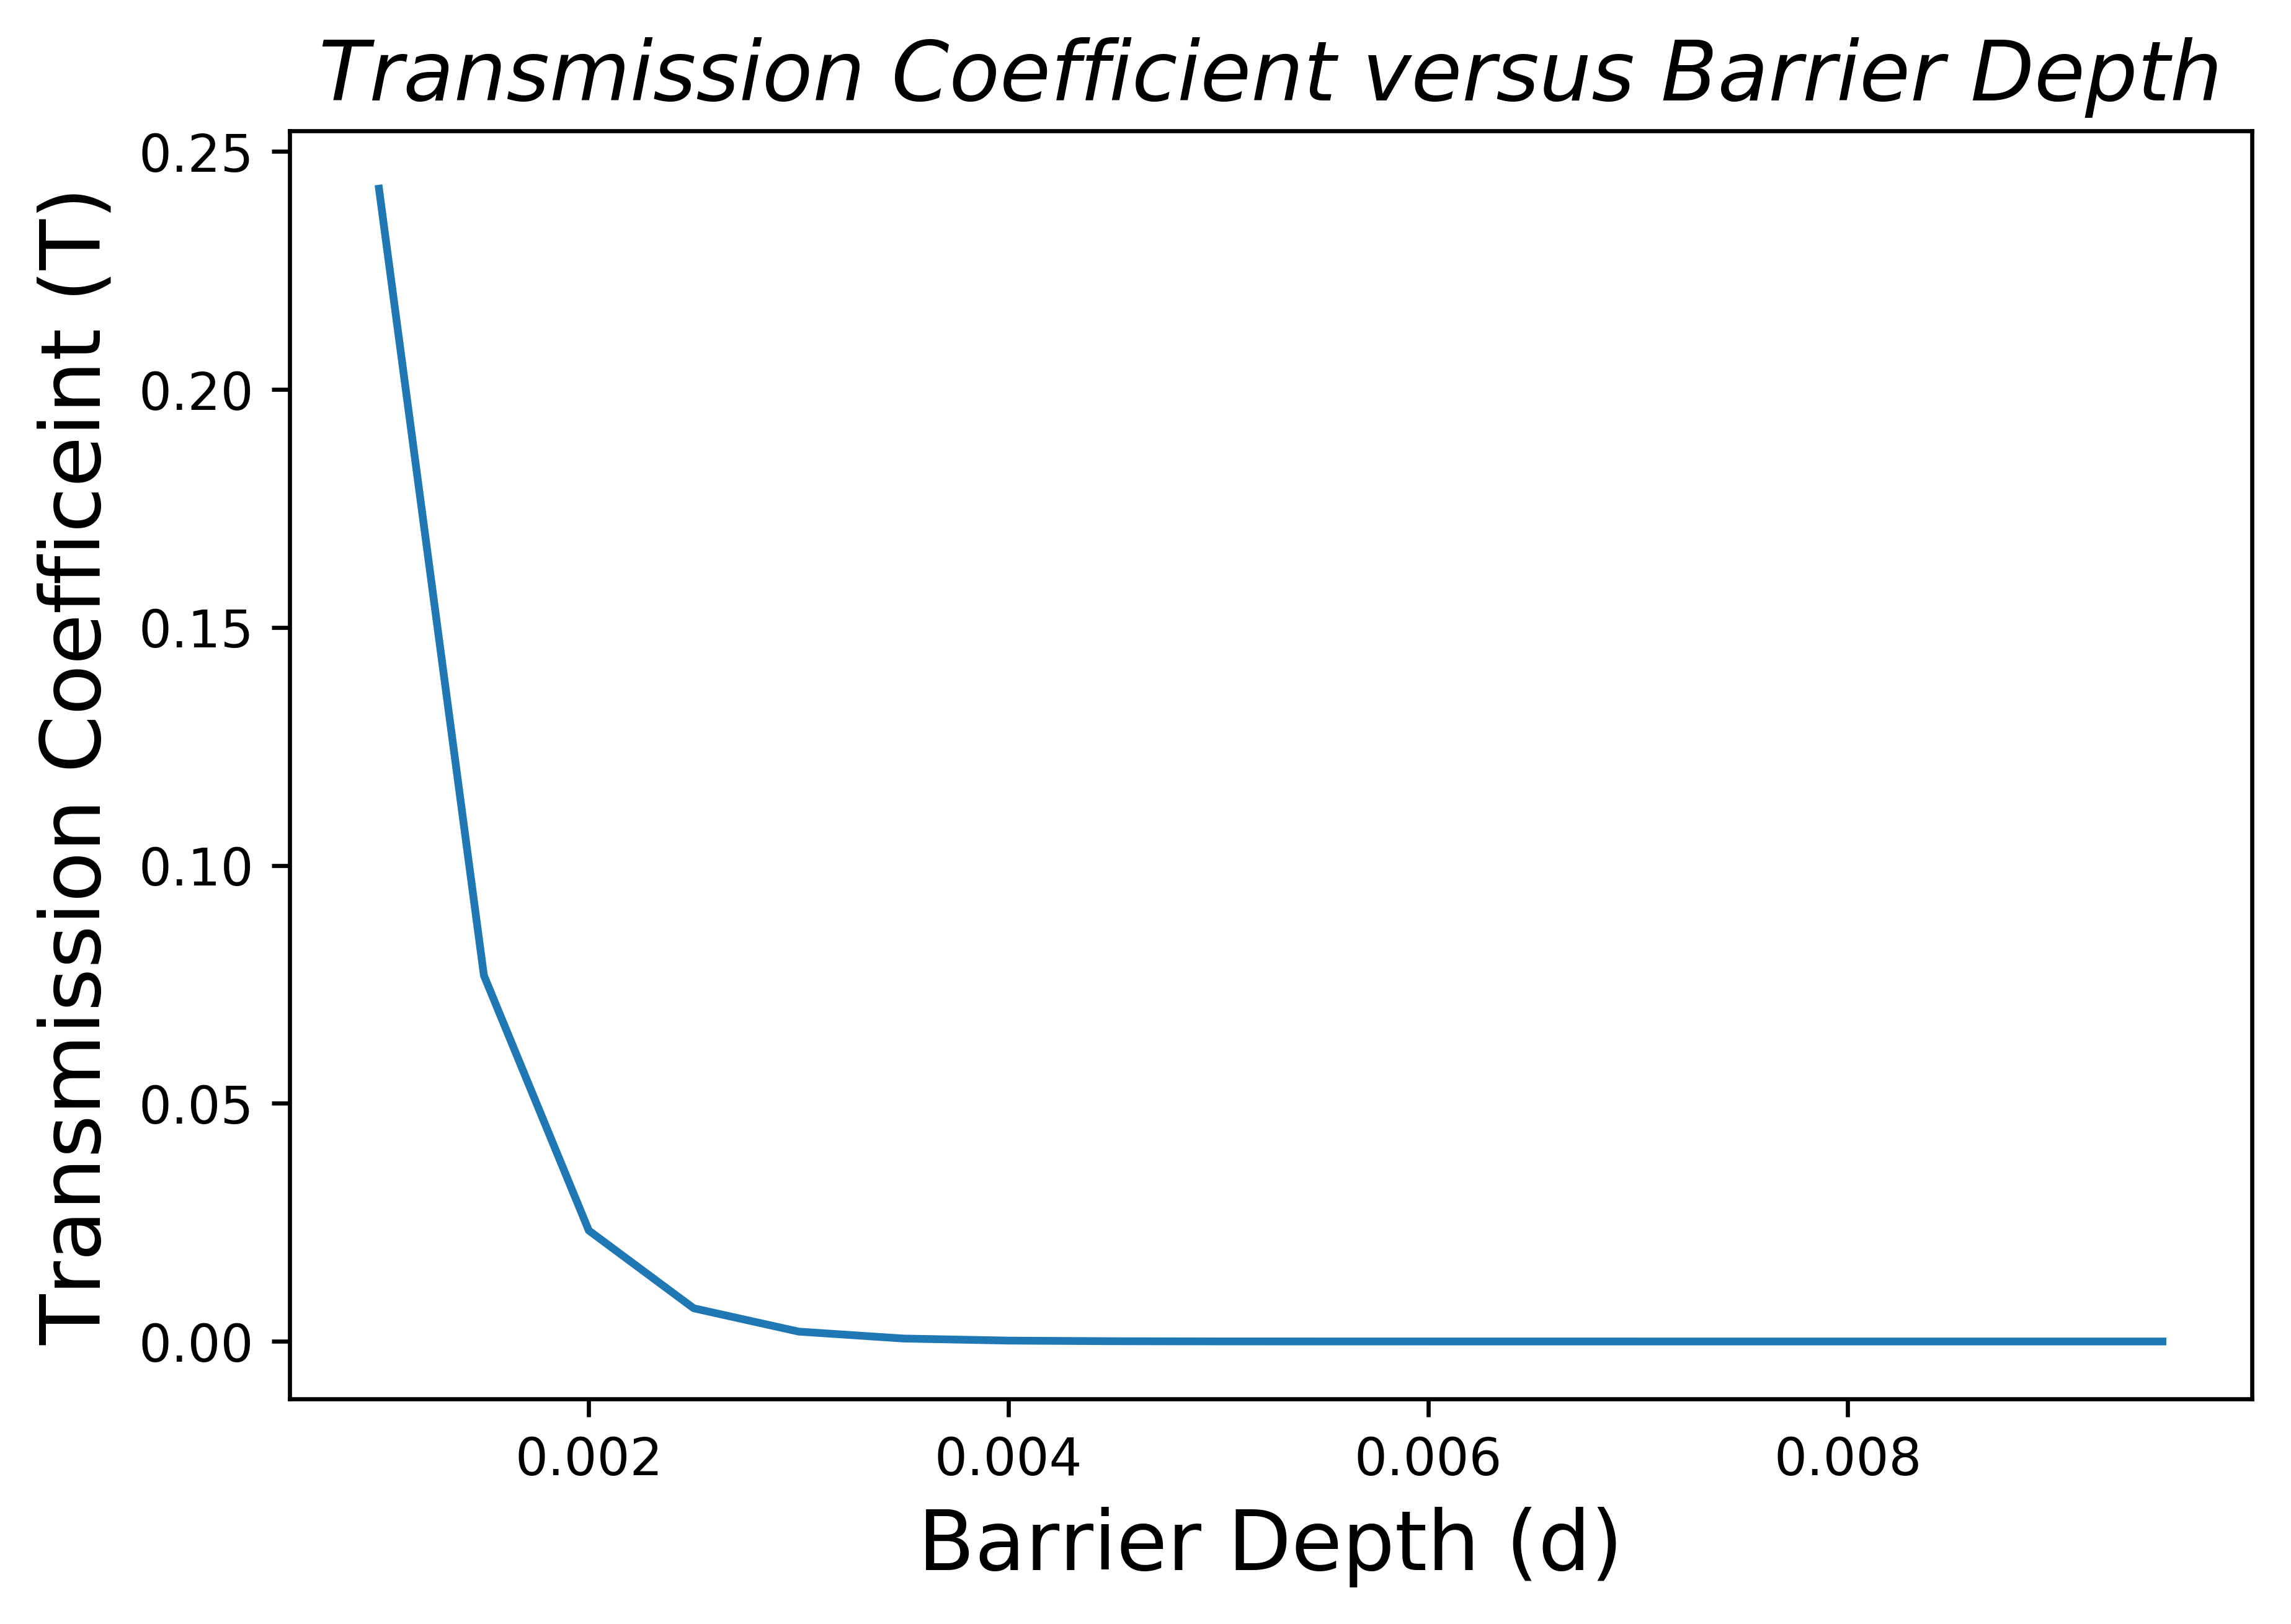
\includegraphics[scale=.5]{TransmissionD}
\small{This plot shows the transmission coefficient of the incident wave $\psi$ against potential barriers of varying depths. As the depth increases the transmission coefficient exponentially decreases.}
\end{figure}
\section{Tunneling Through a Double Barrier: Resonance}
\hspace{\parindent}An interesting consequence of quantum tunneling is that a sort of resonance can occur between potential barriers and wells such that the wave packet is dispersed into many smaller waves being transmitted, reflected, and trapped about the two barriers/wells (see Figure 8). In order to explore this phenomena, the third experiment developed two potential barriers of equal height $(V=9.8\times10^5)$ and depth $(d=.001)$, about a separation $L=.004$ such that the distance between the center of the barriers was $L+d$. Wave packets with varying propagation speeds were then sent at these barriers in order to numerically verify the resonance of the transmission coefficient as a function of $k_0$. The results showed that the transmission coefficient peaked when $k_0=535$ and exponentially decayed on either side (the shape was very Gaussian, see Figure 9). This was expected behavior though, because at higher propagation speeds the majority of the wave packet would simply tunnel through where as at lower speeds the wave packet would not even be able to penetrate the second barrier.
\begin{figure}[H]
\centering
\caption{Wave Packet Distribution for Two Potential Barriers}
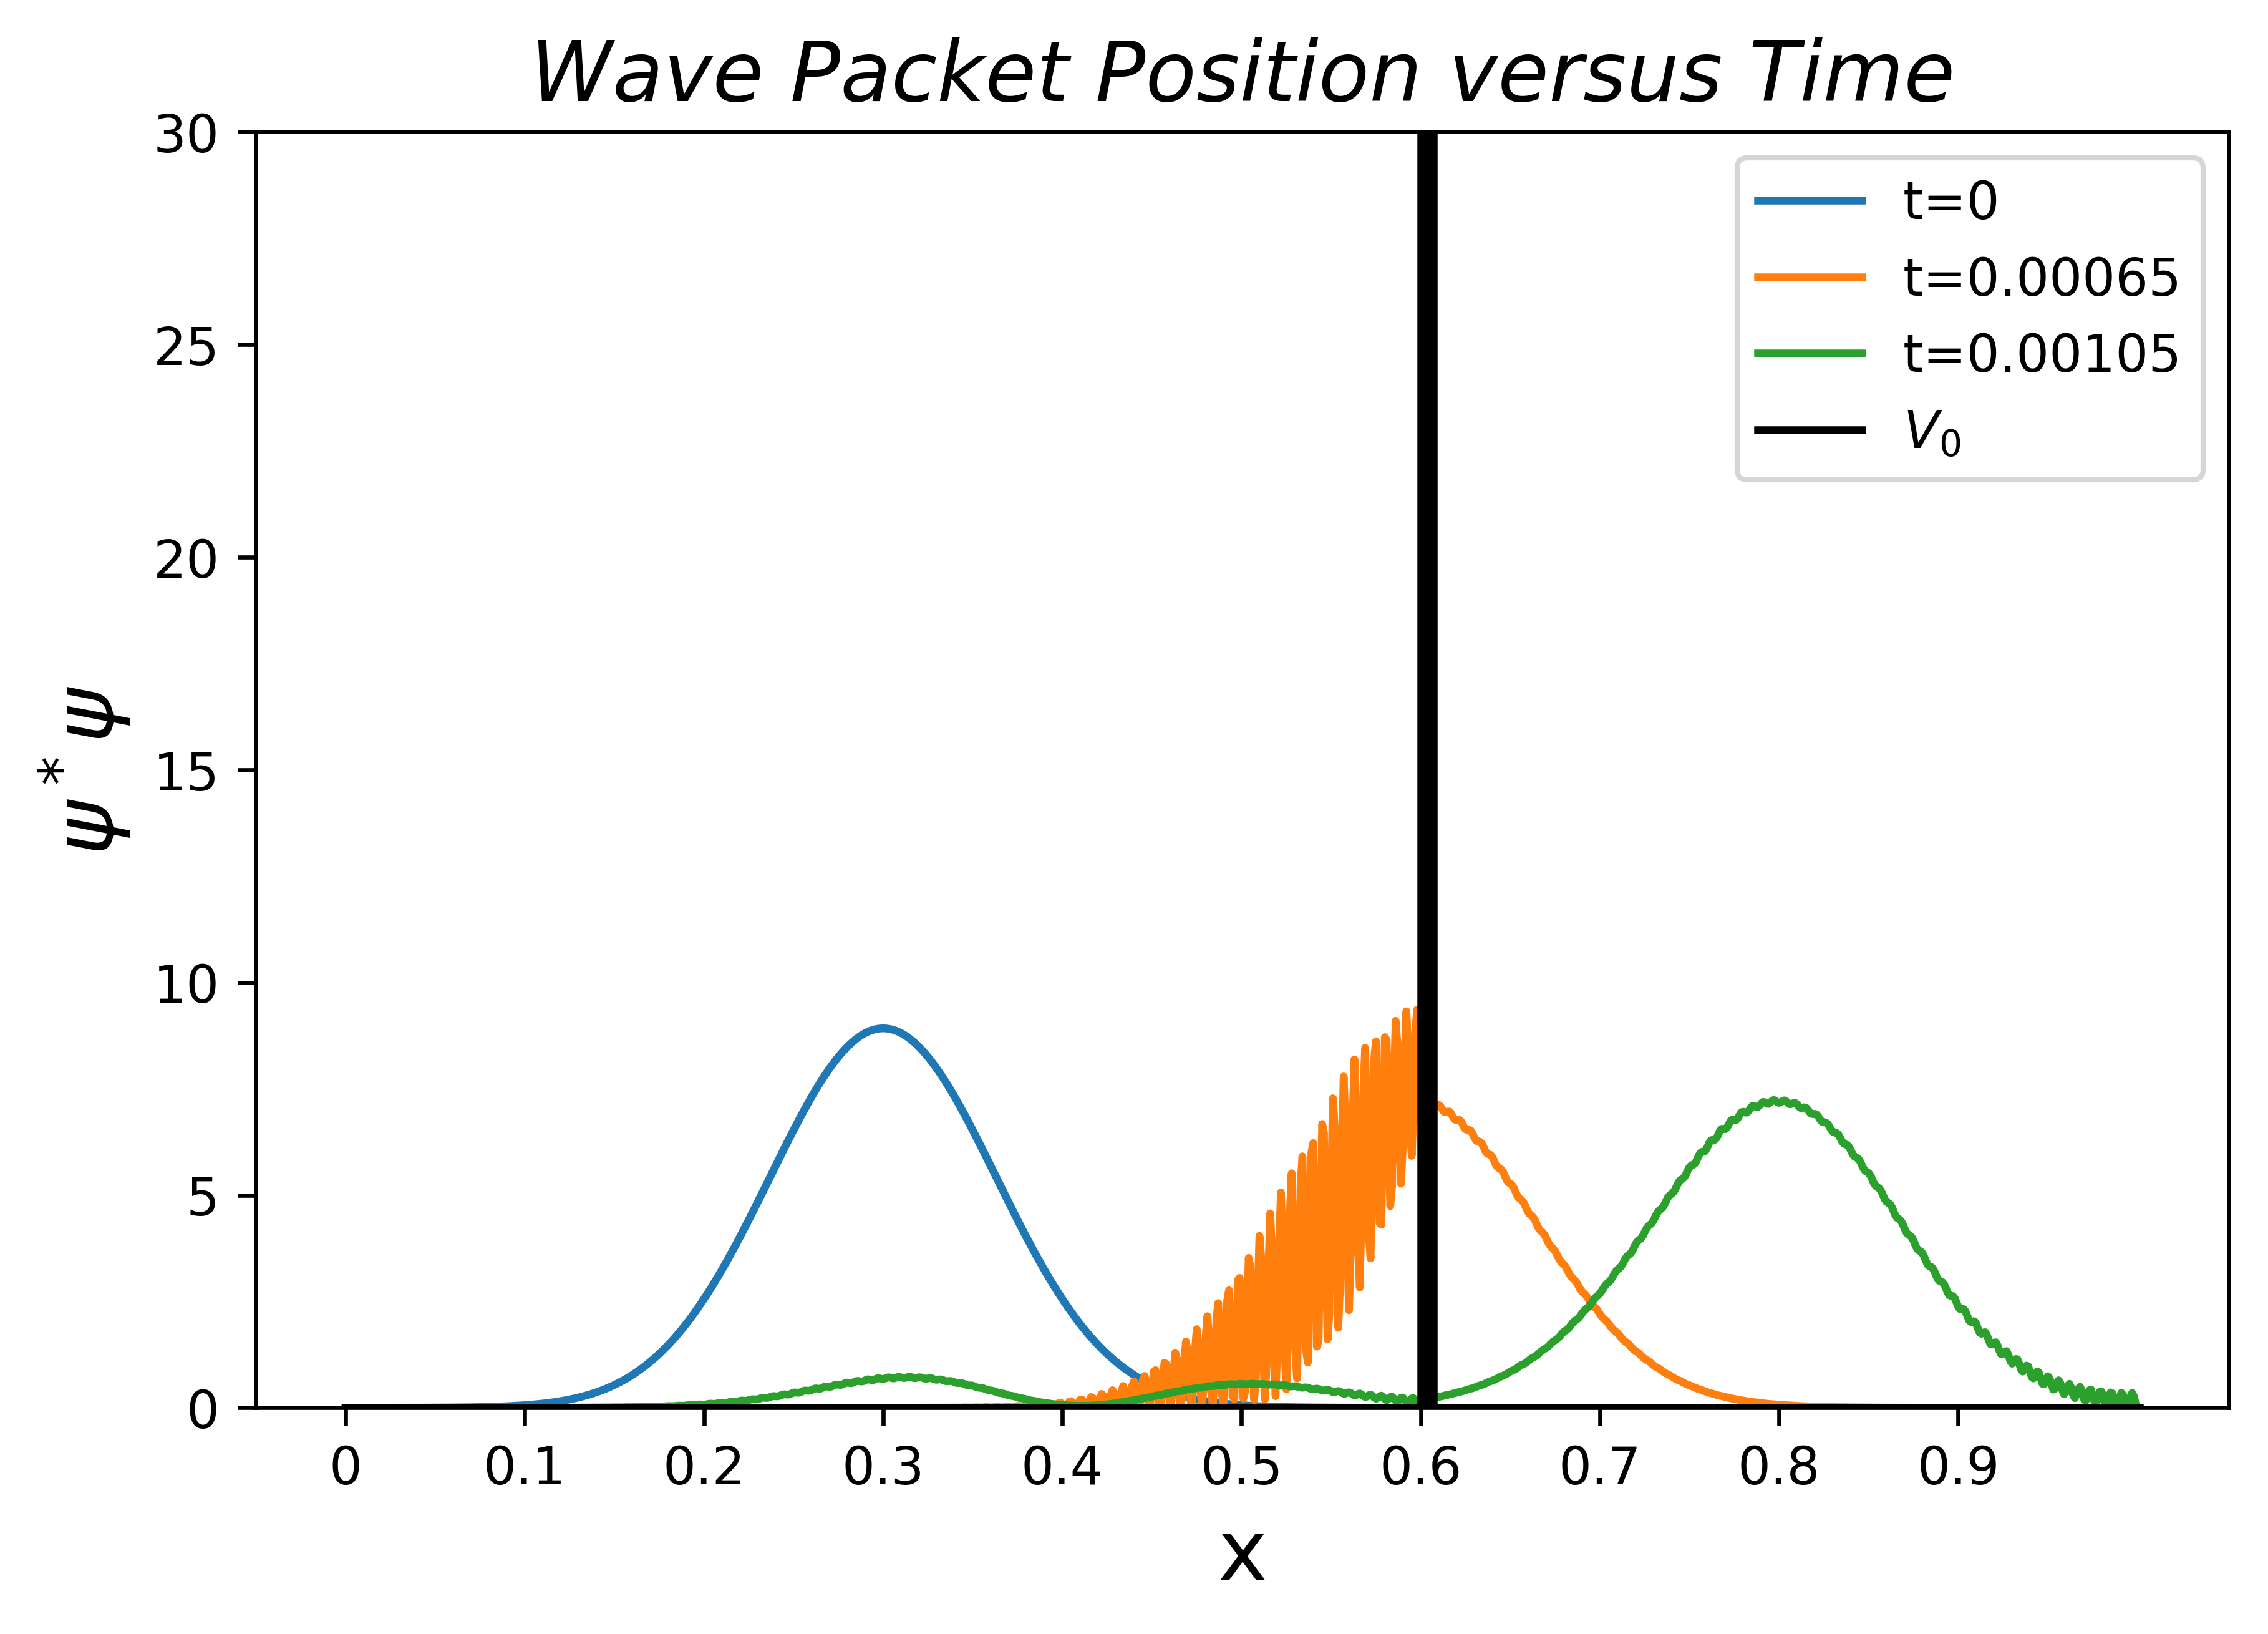
\includegraphics[scale=.5]{Position3}
\small{This plot shows the wave packet distribution of the incident wave $\psi$ against two potential barriers. Looking closely, one can see multiple waves being reflected as a result of resonance between the two barriers.}
%\end{figure}
%\begin{figure}[h]
\centering
\caption{Numeric Transmission Coefficient for Two Potential Barriers}
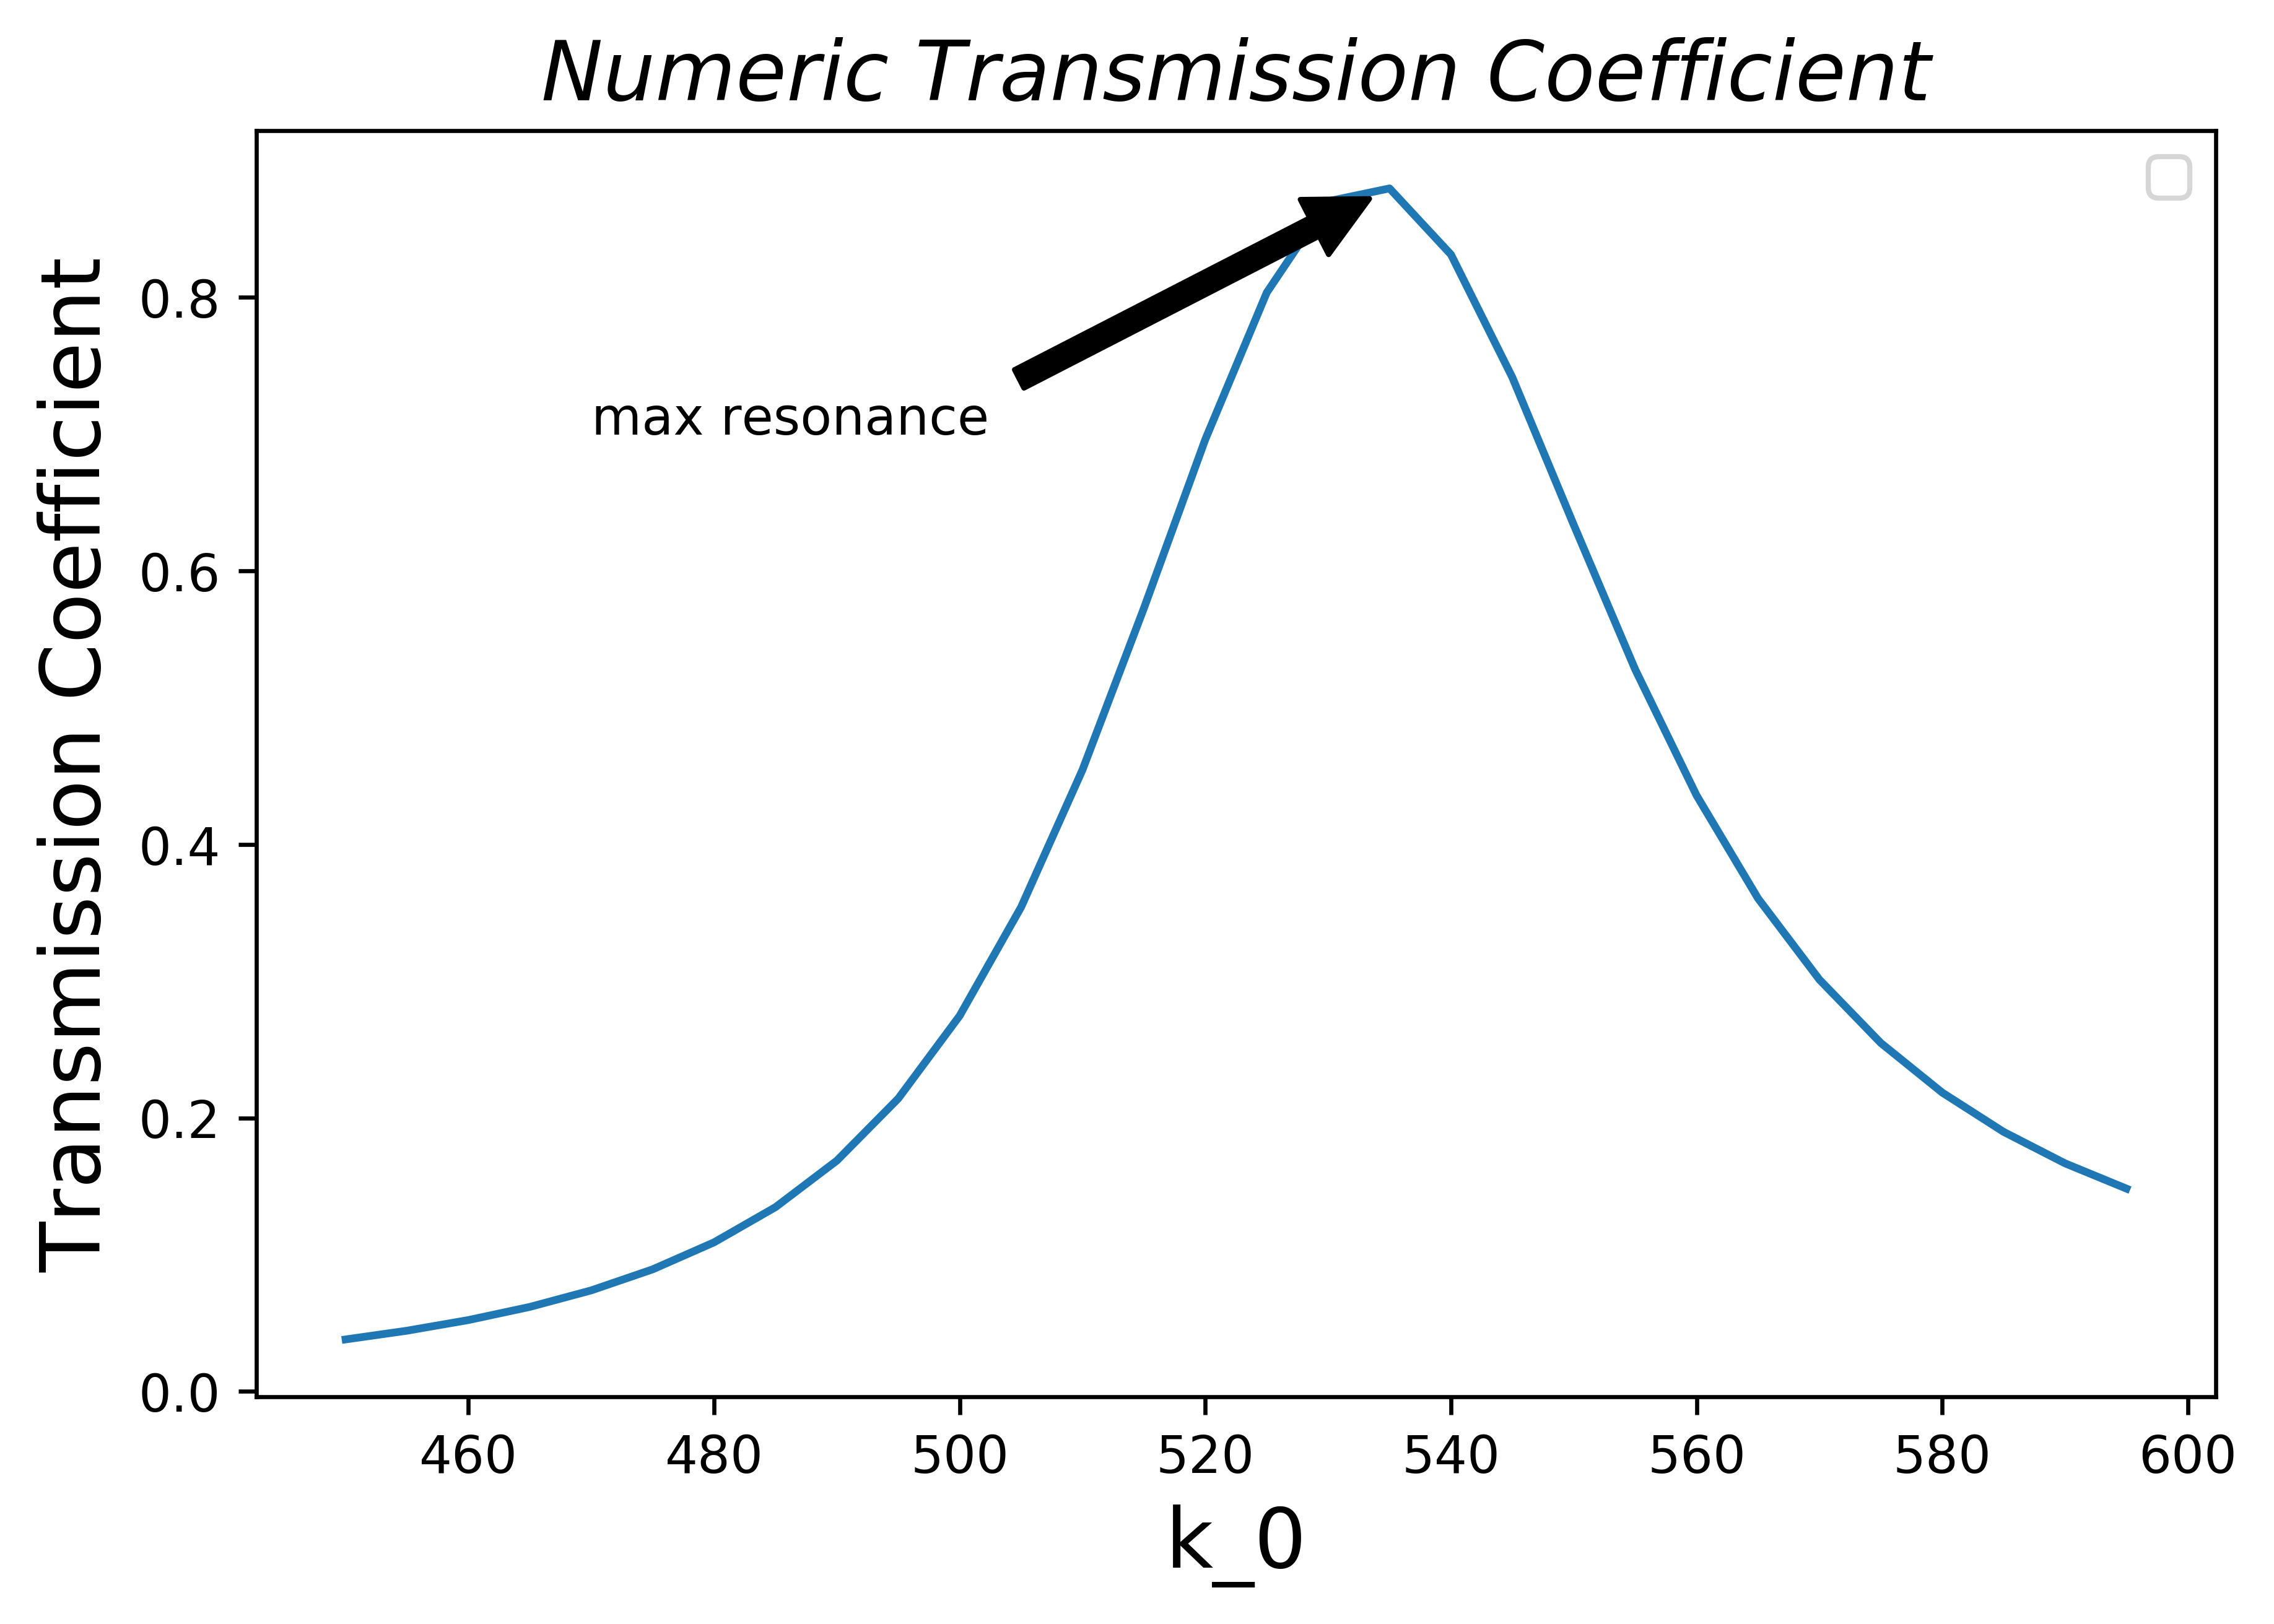
\includegraphics[scale=.5]{T_numeric}
\small{This plot shows the transmission coefficient of the incident wave $\psi$ against two potential barriers. The plot shows a clear peak about $k_0=535$ at which maximum resonance occurs.}
\end{figure}
\section{Scattering By a Potential Well}
\hspace{\parindent} In classical physics, when a wave collides with a potential well with less energy than itself the wave simply passes over. However, quantum mechanically the wave can actually be reflected, similarly to how it can pass through a barrier of greater energy (see Figure 10). The final experiment aimed to explore this phenomena by introducing a single potential well $(V_0=-2.45\times10^5)$ with varying depth $(.001\leq d\leq.01)$ to see how the transmission coefficient would be affected. The speed of the wave packet was also reduced from the typical $k_0=700$ to $k_0=350$, since no reflection would be seen otherwise causing the transmission coefficient to always be 1.
\begin{figure}[hb]
\centering
\caption{Wave Packet Distribution for A Potential Well}
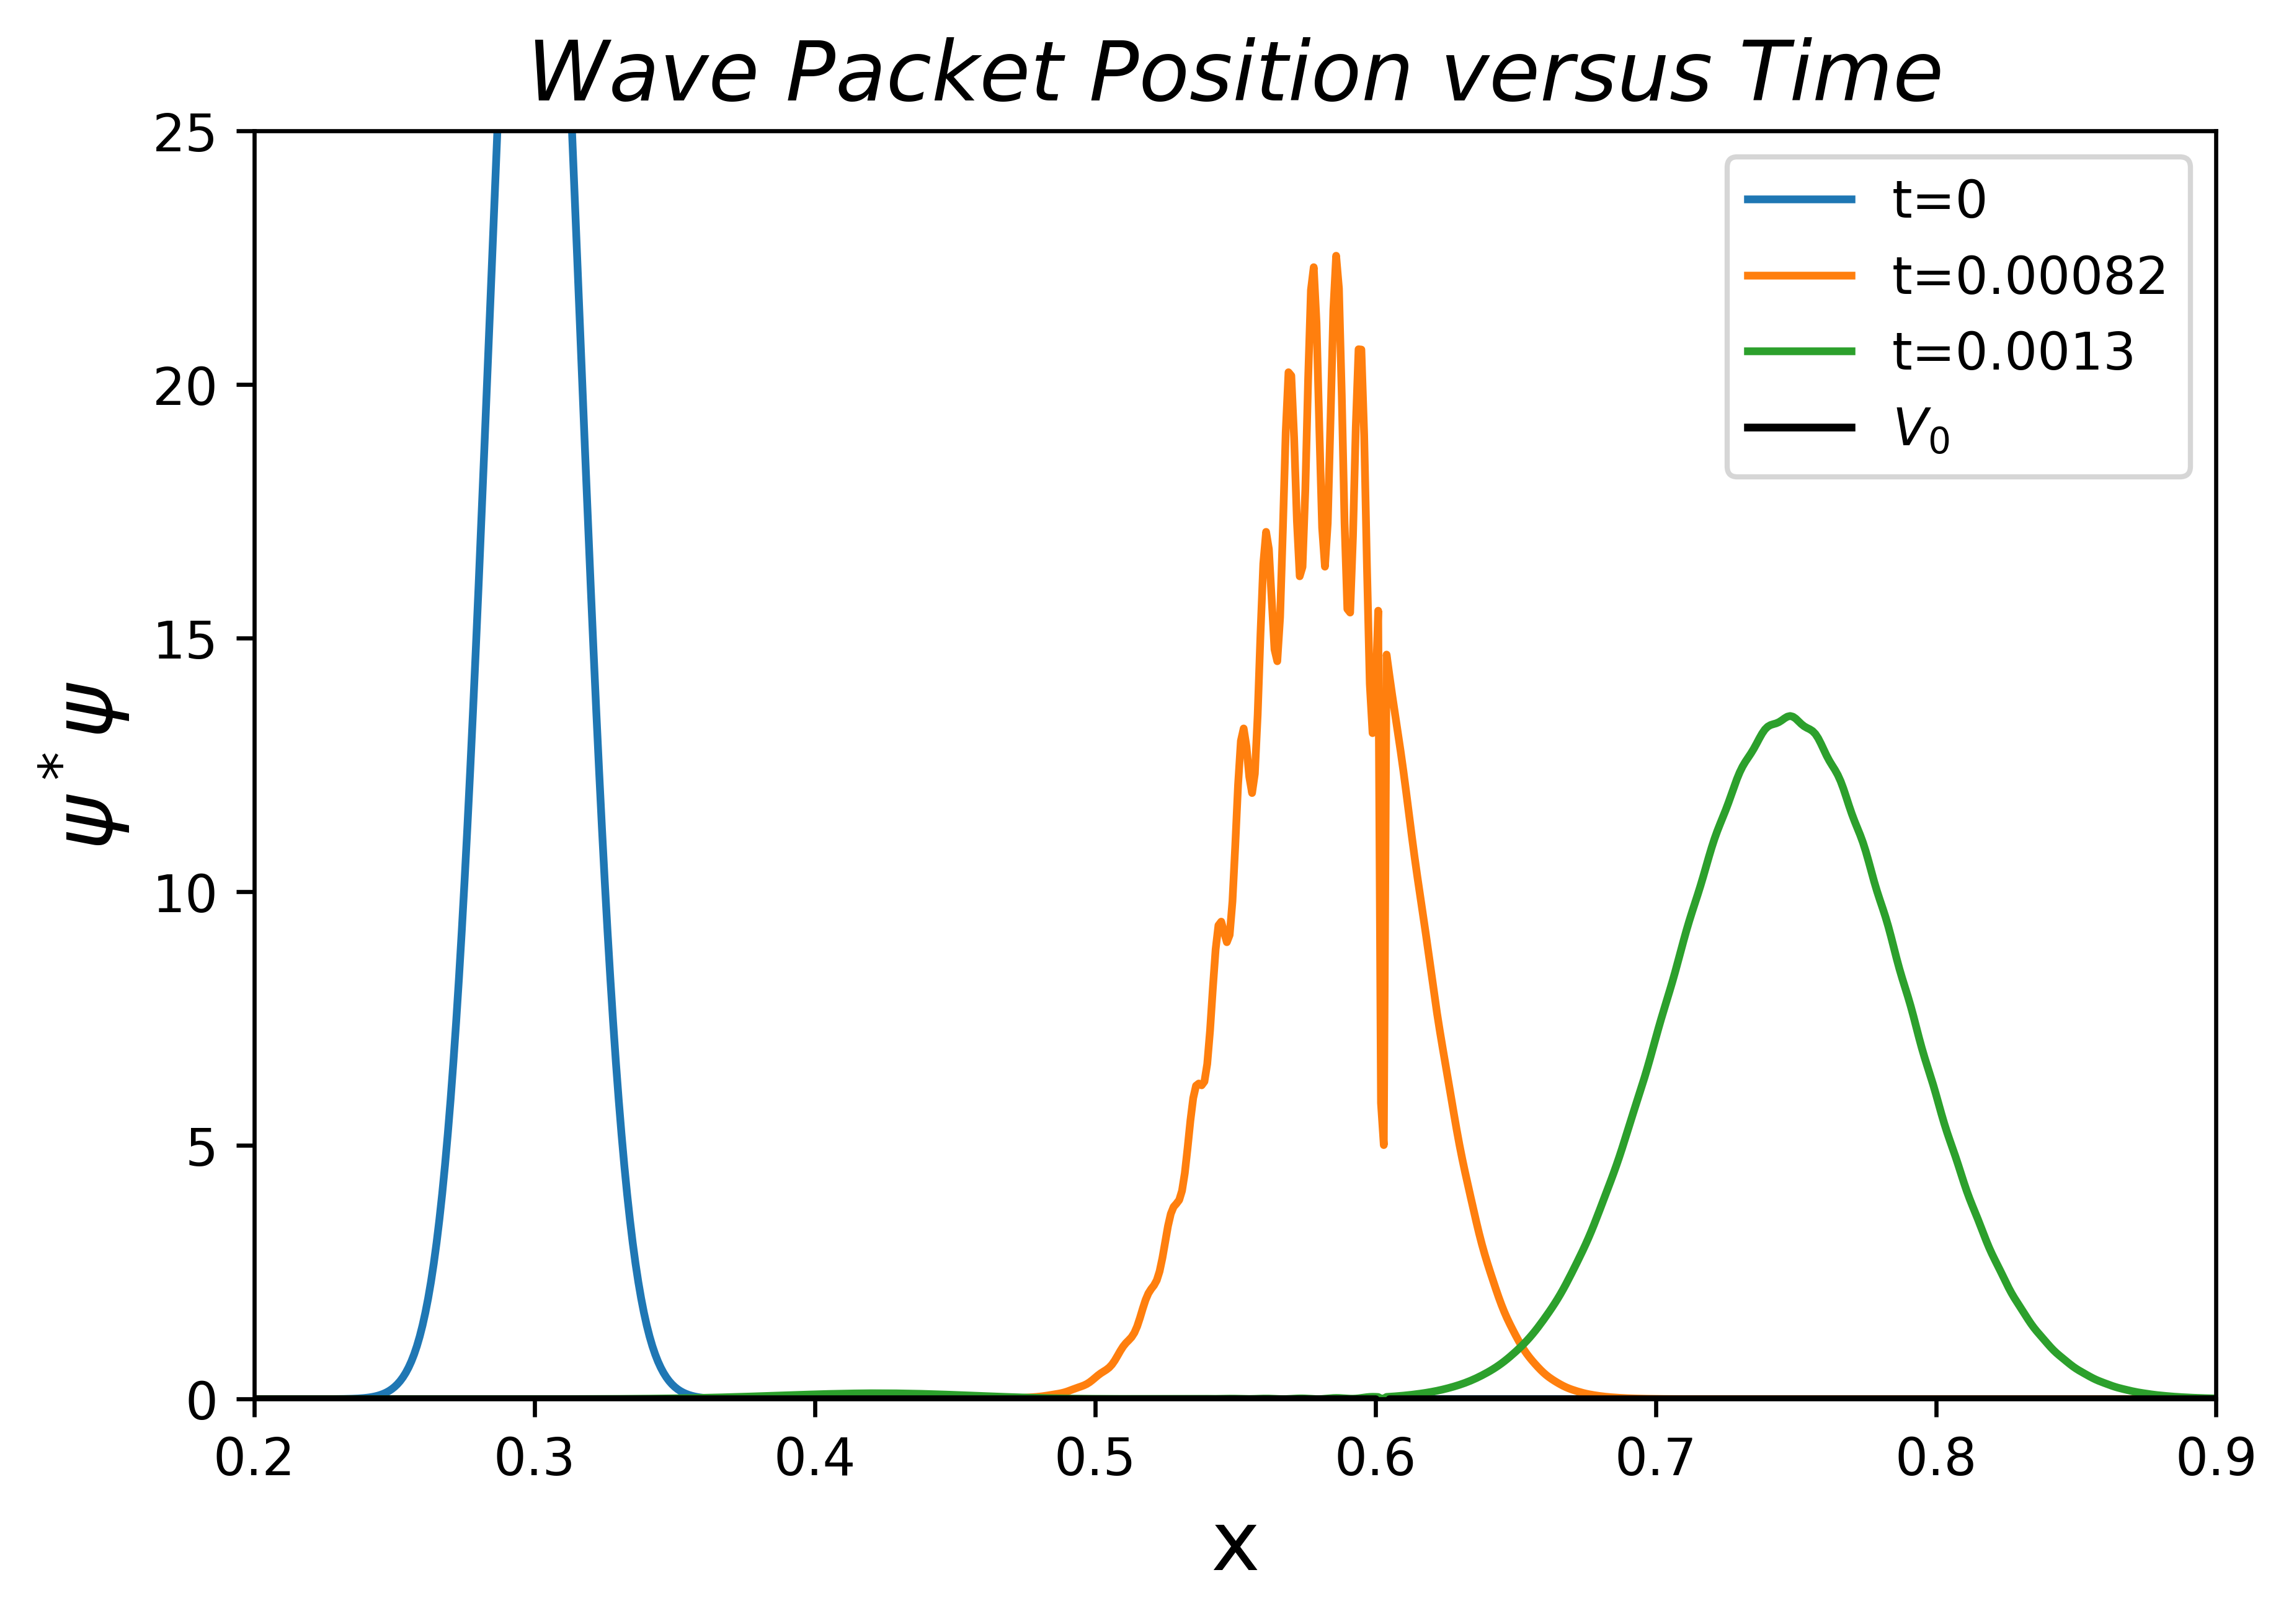
\includegraphics[scale=.5]{Position4}
\small{This plot shows the wave packet distribution of the incident wave $\psi$ against a potential well. About the well there is a sharp decline showing that the particle is not likely at all to be there. Furthermore, about x=.43 a small but distinct reflective wave can be seen!}
\end{figure}
This would be because the energy of the wave would be too 'overpowering' for the well to induce any reflection. It should be noted that an analytic approach - similar to the one found in section 2.2 - can also be utilized to calculate the transmission coefficient. This process reveals that $T$ can be calculated by:
\begin{equation}
	T=\frac{16k_1^2k_2^2}{\left| (k_1+k_2)^2e^{-ik_2a}-(k_2-k_1)^2e^{ik_2a} \right|^2}
\end{equation}
\begin{equation}
	T=\frac{4E(E+V)}{4E(E+V)+V^2\sin^2(k_2a)}
\end{equation}
where $E$, $V$, and $k_1$ are the same variables as found in section 2.2 and $k_2=\frac{\sqrt{2m(E+V)}}{\hbar}$. Plotting the numeric results revealed that there are two peaks instead of only one as seen before (see Figure 11). Notably these peaks occurred at multiples of .004. This is an interesting result, but not completely unexpected because of the $\sin$ term in the analytic solution which would induce cyclic peaks for $T$.
\begin{figure}[hb]
\centering
\caption{Numeric Transmission Coefficient for A Potential Well}
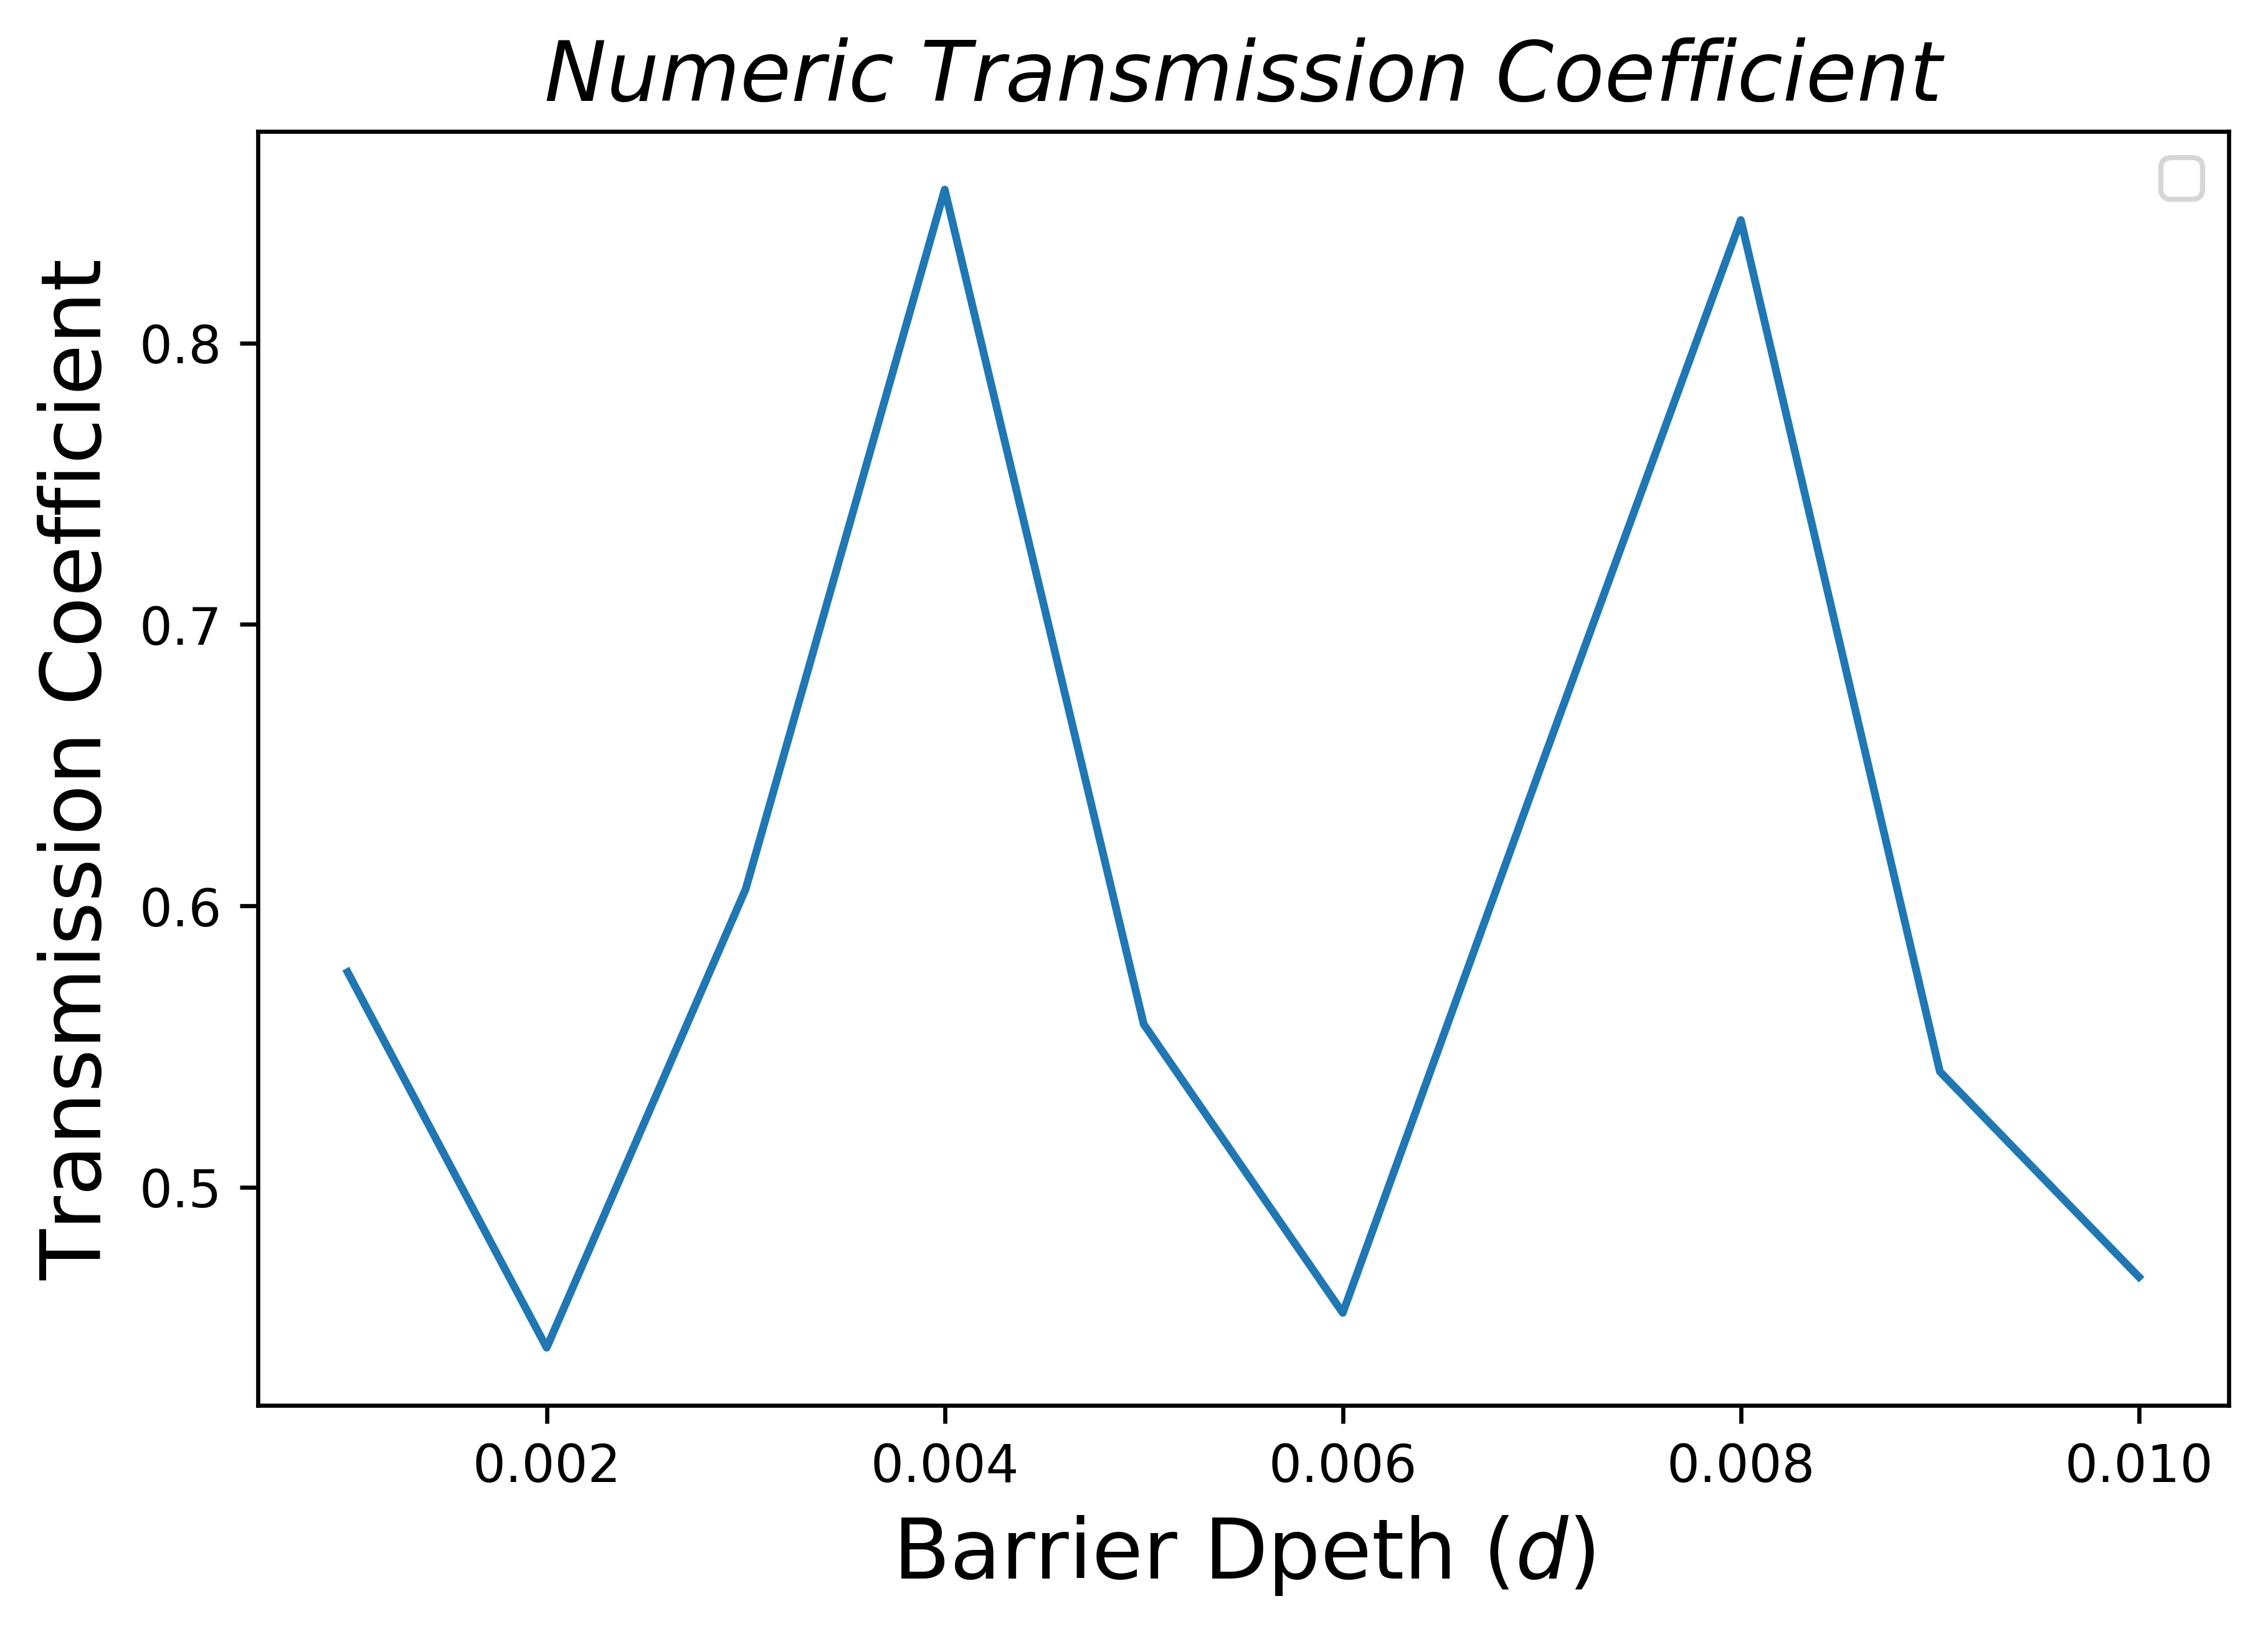
\includegraphics[scale=.5]{T_numericD}
\small{This plot shows the transmission coefficient of the incident wave $\psi$ against a potential well. The plot reveals clear peaks about $d=.004$, $d=.008$ and valleys about $d=.002$, $d=.006$. Notably the peaks correspond to multiples of .004.}
\end{figure}
\section{Conclusion}
In conclusion, each of the experiments were able to produce results that agreed with their analytic counterparts - verifying the analytic conclusions and the integrity of the numeric system. In this sense the overall experiment was certainly successful. Some important highlights included: 
\begin{itemize}
\item demonstrating the wave packet propagation when no potential was present, and verifying that its average position $(<x>)$ and wave distribution $(\sigma(t))$ made physical sense
\item discerning that despite differences in the initial wave packet distribution that their average position and wave distribution grew in the same manner assuming all other factors were equal
\item displaying quantum tunneling through a single potential barrier and verifying that the thicker the barrier the smaller the probability that tunneling occurs
\item numerically calculating the wave propagation speed $(k_0)$ at which the greatest amount of resonance occurs $(k_0=535)$ in the case that $\psi$ is incident to two potential barriers 
\item revealing the production of multiple smaller waves that compose the entire wave packet from the resonance that occurs from $\psi$ being incident to two potential barriers
\item numerically calculating the transmission coefficient in the case that $\psi$ is incident to a potential well and revealing that it has cyclic peaks as a result of the $\sin$ term in the denominator of the analytic result 
\item displaying the physical reflection of a portion of the wave packet due to a potential well, despite this not being possible in classical physics
\end{itemize}
Most notable of all the conclusions of this paper though, has to be the confirmation 
of the need for physics beyond the classical models since they are unable to explain the results of the experiments - wavelike particles passing through potential barriers and being reflected by potential wells. In the past these experiments resulted in the development of quantum tunneling, and consequentially, quantum mechanics at large which has become one of the great pillars of modern physics. Its explanations have lead to the understanding of many phenomena such as nuclear fusion in stars, radioactive decay, and biological mutations as well as the creation of many man-made devices that have changed society such as transistors and tunnel junctions. Given everything that quantum mechanics has already revealed about the nature of the universe, it will undoubtedly lead to many more society changing discoveries.
%%%%%%%%%%%%%%%%%%%%%%%%%%%%%%%%%%%
% New Section
%%%%%%%%%%%%%%%%%%%%%%%%%%%%%%%%%%%
\begin{thebibliography}{9}
\bibitem{latexcompanion} 
\textit{''The One-Dimensional Finite-Difference Time-Domain(FDTD) Algorithm Applied to the Schrodinger Equation''}
James R. Nagel
\end{thebibliography}
\end{document}